\documentclass{ctexbook}

\usepackage{amsthm}
\usepackage{amsmath}
\usepackage{newtxmath}
%\usepackage{ctex} %显示中文的宏包
\usepackage{graphicx}
\usepackage{geometry}
\geometry{left=3cm,right=3cm,top=3cm,bottom=2cm}
%\numberwithin{equation}

%\usepackage{times}
%\usepackage{fontspec, xunicode, xltxtra}    % 字体设置包
%\setmainfont{Times New Roman}


%\renewcommand\theequation{\thechapter-\arabic{equation}}

\newtheorem{thm}{定理}[section]
\newtheorem{lem}[thm]{引理}
\newtheorem{prop}[thm]{性质}
\newtheorem{cor}[thm]{推论}
\newtheorem{conj}[thm]{猜想}
\newtheorem{rem}[thm]{注}
\newtheorem{propo}[thm]{命题}

\begin{document}
\author{Bruce Sagan}
\title{Art of counting(计数的艺术)}
\date{}
\maketitle
\newpage
\chapter{基本计数}
\begin{center}
(伍思懿 \quad 翻译)
\end{center}


本章我们将了解最基础的集合计数方法. 尽管这些方法是比较基础的, 但它们预示着会有更复杂的事情发生. 我们用$\mathbb{Z}$表示整数,
除非另有说明, 否则通常假设参数如$n$和$k$为整数. 对于非负整数和正整数, 我们分别使用符号$\mathbb{N}$和$\mathbb{P}$来表示,
并用$\mathbb{Q}$、$\mathbb{R}$和$\mathbb{C}$分别代表有理数、实数和复数. 最后, 每当使用基数集时, 我们都会假设它是有限的.

\section{集合的加法与乘法原则}

集合的加法与乘法原则是许多枚举的基础. 我们之后会看到它们在普通和指数生成函数中的各种推广. 尽管这些规则证明起来微不足道,
但我们将给出证明, 因为这个结果很有用. 给定一个有限集 $S$, 我们用符号$\# S$ 或者 $|S|$来表示它的基数, 我们也用
$S \uplus T$ 来表示 $S$ 和 $T$ 的不相交并, 使用这个符号意味着不相交. 最后, 我们将笛卡尔积记为
$$ S \times T=\{(s, t) \mid s \in S, t \in T\}.$$

\begin{lem}
令$S$, $T$为有限集.

\noindent(1)\ (加法原则)如果 $S \cap T=\varnothing$, 则
$$|S \uplus T|=|S|+|T|.$$
(2)\ (乘法原则)对任意有限集, 有
$$|S \times T|=|S| \cdot|T|.$$
\end{lem}


\begin{proof}
$S=\left\{s_{1}, \ldots, s_{m}\right\}$ , $T=\left\{t_{1}, \ldots, t_{n}\right\} $. 如果$S$和$T$是不相交的, 则
$S\uplus T=\left\{s_{1}, \ldots, s_{m}, t_{1}, \ldots, t_{n}\right\}$, 因此$|S \uplus T|=m+n=|S|+|T|$.
对任意集合$S$, $T$, 将$S \times T$的元素放入一个$m \times n$的矩阵, 其中位于$(i, j)$ 的元素为 $\left(s_{i}, t_{j}\right)$.
计算这个矩阵元素的个数可得$|S \times T|=m n=|S| \cdot|T|$.
\end{proof}


%\noindent
%\textbf{引理\ 1.1.1.}\textsl{令$S$, $T$为有限集. }
%
%\noindent
%\textsl{(1)\ (加法原则)如果 $S \cap T=\varnothing$ , 则
%$$|S \uplus T|=|S|+|T|.$$
%(2)\ (乘法原则)对任意有限集, 有
%$$|S \times T|=|S| \cdot|T|.$$
%证明:}$S=\left\{s_{1}, \ldots, s_{m}\right\}$ , $T=\left\{t_{1}, \ldots, t_{n}\right\} $. 如果S和T是不相交的, 则
%$S\uplus T=\left\{s_{1}, \ldots, s_{m}, t_{1}, \ldots, t_{n}\right\}$, 因此$|S \uplus T|=m+n=|S|+|T|$.
%对任意集合$S$, $T$, 将$S \times T$的元素放入一个$m \times n$的矩阵, 其中位于$(i, j)$ 的元素为 $\left(s_{i}, t_{j}\right)$.
%计算这个矩阵元素的个数可得$|S \times T|=m n=|S| \cdot|T|$. \hfill\qedsymbol
%%$\hfill\qedsymbol$

在组合选择问题中, 我们通常只能做一个选择或做另一个, 或者两者都做. 假设做第一个选择有$m$种方法, 做第二个选择有$n$种方法.
如果没有相同的选择, 那么加法原则告诉我们方法数是$m+n$. 如果做第一个选择对做第二个选择没有影响,
那么由乘法原则可得做第一个选择有$mn$种, 然后再做第二个选择. 所以在实践中, 人们用“或”代表加法, 用“和”代表乘法.

%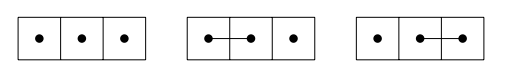
\includegraphics[width=3.00in,height=0.50in]{./fig1/figure1.1.jpg}

我们将用所有组合学中最著名的序列之一:斐波那契数列来说明这些概念. 有时也这样说, 关


\begin{figure}
    \centering
    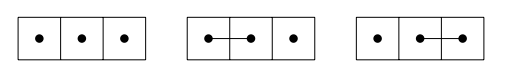
\includegraphics[scale=0.8]{./fig1/figure1.1.jpg}
    \caption{$\mathcal{T}_{3}$}\label{fig-1}
\end{figure}





\noindent
于这个序列有一个有趣的故事
(多少有点不可能). 一开始有一对未成熟的兔子, 一雄一雌, 兔子要一个月才能成熟. 在之后的每一个月, 一对兔子会产下一对幼兔,
一雄一雌. 如果兔子只和它们的生育伙伴繁殖并长生不老(就像我说的, 这个故事有点不太可能), 那么在第$n$个月初有多少对兔子?
我们称这个数字为$F_{n}$. 为了方便, 我们令$F_{0}=0 $. 因为我们一开始只有一对, $F_{1}=1$. 在第二个月初, 这一对已经成熟,
但没有生产后代, 所以$F_{2}=1$. 在后面的月份中, 兔子的数量是之前月份所有的兔子加上这个月新出生的兔子, 记为$F_{n-1}$.
新生的对数等于前一个月的成熟兔子对数, 等于前一个月的配对总数, 为$F_{n-2}$. 因此, 用加法原则可得,
\begin{equation}
F_{n}=F_{n-1}+F_{n-2} \text { 对 } n \geqslant 2 \text { 有 } F_{0}=0 \text { 及 } F_{1}=1.
\end{equation}
因为我们令$F_{0}=0 $ , 故我们的递归公式从$n=2$ 开始而不是 $n=3$. $F_{n}$就称作斐波那契数. 同样, 要注意一些作者将这个数列定义为
\begin{equation}
f_{0}=f_{1}=1 \quad \text { 且  } \quad  f_{n}=f_{n-1}+f_{n-2}, \quad  n \geqslant 2.
\end{equation}
因此, 我们必须明确文章讨论的是哪一种斐波那契数列.

人们可能会想, 除了上面的递归公式之外, 是否还有一个显式的$F_{n}$公式. 这样的表达式是存在的,
尽管从我们目前所做的来推导出它还很困难. 事实上, 我们需要在第三章中讨论的生成函数的理论来推导它.

另一个我们需要了解的是$F_{n}$的组合解释. 非负整数序列$a_{0}, a_{1}, a_{2}, \ldots$的组合解释是一个集合的序列
$S_{0}, S_{1}, S_{2}, \ldots$ , 其中, 对所有$n$有$\# S_{n}=a_{n}$. 这样的解释常常能得到关于原序列的非常漂亮和直观的证明,
因此是非常可取的. 有人可能会说, 兔子的故事已经给出了这样的解释, 但我们想要更适合数学操作的东西.

假设我们有一排方块. 我们给出两种类型的瓷砖:覆盖两个方块的双方块和覆盖一个方块的单方块. 则这一排方块的平铺为:每个方块被覆盖一次的
瓷砖集. 令$\mathcal{T}_{n}$为一排$n$个的平铺集合. 图\ref{fig-1}中列出了$\mathcal{T}_{3}$的所有元素. 平铺和斐波那契数列之间有一个简单的关系.
    \begin{thm}
   	      对$n \geqslant 1$,  有
   		  $$F_{n}=\# \mathcal{T}_{n-1}.$$
    \end{thm}
    \begin{proof}
    	 只需证方程两边满足相同的初始条件和递归关系就足够了. 当不包含方块时, 它只有空的覆盖, 故$\mathcal{T}_{0}=1=F_{1}$.
    	 当有一个方块的时候, 它只能被一个单方块覆盖, 故$\mathcal{T}_{1}=1=F_{2}$. 对于递归, $\mathcal{T}_{n}$
    	 中的平铺可分为两种类型:以单方块结尾的平铺和以双方块结尾的平铺. 去掉最后的瓷砖我们可以得到这两种平铺分别与
    	 $\mathcal{T}_{n-1}$和$\mathcal{T}_{n-2}$ 构成双射. 因此, 可得$\# \mathcal{T}_{n}=\# \mathcal{T}_{n-1}+\# \mathcal{T}_{n-2}$.
    \end{proof}
    为了展示一个好的组合解释的威力, 我们现在给出一个$F_{n}$的恒等式的简单证明. 这样的恒等式有很多. 比如, Benjamin和Quinn的书[10].
    \begin{cor}
    	对 $m \geqslant 1$ 及 $n \geqslant 0$, 有
    		$$F_{m+n}=F_{m-1} F_{n}+F_{m} F_{n+1}.$$
    \end{cor}
    \begin{proof}
    	由之前的定理, 左边为$m+n-1$个方块的平铺数. 故我们只需证右边也是如此. 给这些方块从左至右记为$1, \ldots, m+n-1$.
    	记$\mathcal{T}_{m+n-1}=\mathcal{S} \uplus \mathcal{T}$, 其中$\mathcal{S}$是所有以双方块覆盖第$m-1$ 和第$m$个方块的平铺的集合,
    	$\mathcal{T}$是所有第$m-1$ 和 第$m$个在不同瓷砖覆盖下的平铺的集合. $\mathcal{T}$中的平铺事实上是由两个平铺组成的,
    	第一个覆盖了前面$m-1$个方块, 而第二个覆盖了最后的$n$个方块. 故由乘积规则得$|\mathcal{T}|=\left|\mathcal{T}_{m-1}\right| \cdot\left|\mathcal{T}_{n}\right|=F_{m} F_{n+1} $.
    	将$\mathcal{S}$中的平铺删掉包含第$m-1$ 和第$m$个方块的双方块, 同样, 将每个平铺拆成两个, 第一个覆盖前$m-2$个方块, 而第二个覆盖后$n-1$个方块.
    	取基数可得$|\mathcal{S}|=F_{m-1} F_{n} $, 最后由加法原则即得证.
    \end{proof}
刚才给出的论证被称为\textsl{组合证明}, 因为它涉及到对离散对象的计数. 在接下来的过程中, 我们将遇到其他有用的证明技巧.
但组合证明通常被认为是最令人愉快的, 部分原因是它们比只涉及形式操作的演示更具启发性.

\section{排列与词}
在考虑枚举问题时, 确定所考虑的对象是否有序总是很重要的. 在这一节中, 我们将考虑最基本的有序结构, 即排列和词.

若集合$S$有$\# S=n$, 则$S$的一个\textsl{排列}就是通过把$S$的元素按一定顺序列出来得到的一个序列$\pi=\pi_{1} \ldots \pi_{n}$.
如果$\pi$是一个排列, 我们通常用$\pi_{i}$来表示$\pi$的第$i$个元素, 同样地, 对于其他有序结构也是如此. 我们用$P(S)$
表示$S$所有排列的集合, 例如
$$P(\{a, b, c\})=\{a b c, a c b, b a c, b c a, c a b, c b a\}.$$
显然, $\# P(S)$只取决于$\# S $. 故我们通常选择正则$n$元集
$$[n]=\{1,2, \ldots, n\}.$$
我们也考虑$S$的\textsl{$k$-排列}, 即由$S$的$k$个不同元素通过线性排序得到的序列$\pi=\pi_{1} \ldots \pi_{k}$.
这里$k$被称为排列的\textsl{长度}, 记为$\ell(\pi)=k$. 我们用同样地名称和符号来表示其他有序结构. $S$的所有$k$-排列的集合记为$P(S, k)$. 以实例说明,
$$P(\{a, b, c, d\}, 2)=\{a b, b a, a c, c a, a d, d a, b c, c b, b d, d b, c d, d c\}.$$
特别的, 如果$\# S=n$, 则$P(S, n)=P(S)$. 并且, 当$k>n$时, $P(S, k)=\varnothing$, 因为在这种情况下, 不可能从只有n个元素的集合中选出k个不同的元素.
以及$P(S, 0)=\{\epsilon\}$, 其中$\epsilon$是空序列.

为了计算排列, 引入下面的符号会很方便. 给定非负整数$n$,  $k$, 我们可以生成降阶
$$n \downarrow_{k}=n(n-1) \ldots(n-k+1)$$
注意, $k$表示乘积中因数的数量.
    \begin{thm}
    	\textsl{对}$n, k \geqslant 0$, \textsl{我们有}
    		$$\# P([n], k)=n \downarrow_{k}.$$
    		\textsl{特别地}
    		$$\# P([n])=n !$$
    \end{thm}
    \begin{proof}
    	因为$P([n])=P([n], n)$, 故证明第一个公式就足够了, 给定$\pi=\pi_{1} \ldots \pi_{k} \in P([n], k)$, 有$n$种方法取$\pi_{1}$.
    	因为$\pi_{2} \neq \pi_{1}$, 故$\pi_{2}$还有$n-1$种取法, 由于$\pi_{2}$的取法与$\pi$中实际所选元素无关, 所以可以继续这样做, 应用一个改进后的乘积规则即得证.
    \end{proof}
注意, 当$0 \leqslant k \leqslant n$时, 记
\begin{equation}
n \downarrow_{k}=\frac{n !}{(n-k) !}.
\end{equation}
但当$k>n$时, 尽管乘积$n \downarrow_k$不能表示为阶乘的商, 但其仍有意义. 事实上, 如果$k>n$, 则0也是一个因数, 故$n \downarrow_{k}=0$.
这与$P([n], k)=\varnothing $相符. 在特殊情况$k=0$时, $n \downarrow_{k}=1$. 因为它是一个空的乘积. 同样, 这反映了$\# P([n], 0)=$ $\{\epsilon\}$中的组合逻辑.

在组合问题中需要注意的另一件事是元素是否允许重复. 在排列中没有重复, 但是当它们被允许的情况也很有趣.
一个集合$S$上的$k$-词是$w=w_{1} \ldots w_{k}$的序列, 其中对任意$i$有$w_{i} \in S$. 注意, 这里并没有假设$w_{i}$是不同的.
我们把$S$上的$k$-词的集合记为$P((S, k))$. 注意, 使用双括号表示允许重复. 还要注意到$P(S, k) \subseteq P((S, k))$,
但通常其包含的内容很严格, 例如
$$P((\{a, b, c, d\}, 2))=P(\{a, b, c, d\}, 2) \uplus\{a a, b b, c c, d d\}.$$
下一个结果的证明与定理1.2.1的证明几乎相同, 因此留给读者来做.
    \begin{thm}
    	\textsl{对}$n, k \geqslant 0$ \textsl{有}
    		$$\# P(([n], k))=n^{k}.$$
    \end{thm}

\section{组合与子集}
现在我们将考虑上一节中所研究组合对象的无序版本. 他们有时被称为组合, 尽管读者可能知道他们更熟悉的名字:子集.

给定一个集合$S$, 我们用$2^{S}$表示$S$的所有子集的集合. 注意, $2^{S}$是一个集合, 而不是一个数字. 例如,
$$2^{\{a, b, c\}}=\{\varnothing,\{a\},\{b\},\{c\},\{a, b\},\{a, c\},\{b, c\},\{a, b, c\}\}.$$
使用这种表示方法的原因可以通过下面的结果来说明.
     \begin{thm}
     	\textsl{对}$n \geqslant 0$\textsl{我们有}
     		$$\# 2^{[n]}=2^{n}.$$
     \end{thm}
     \begin{proof}
     	根据定理1.2.2, 得$2^{n}=\# P((\{0,1\}, n))$. 所以我们只需找到如下双射
     	$$f: 2^{[n]} \rightarrow P((\{0,1\}, n)),$$
     	这是一个典型的例子. 特别地, 如果$S \subseteq[n]$, 那么我们让$f(S)=w_{1} \ldots w_{n}$, 其中, 对所有$i$,
     	$$
     	w_{i}=\left\{\begin{array}{ll}
     	1 & \text { 如果\ } i \in S,\\
     	0 & \text { 如果\ } i \notin S.
     	\end{array}\right.
     	$$
     	要证明$f$是一个双射, 只要找到它的逆就够了. 如果$w=w_{1} \ldots w_{n} \in P((\{0,1\}, n))$, 则设$f^{-1}(w)=S$, 其中, 当$w_{i}=1$
     	时$i \in S$, $w_{i}=0$时$i \notin S$, $1 \leqslant i \leqslant n $. 很容易验证$f \circ f^{-1}$ 和 $f^{-1} \circ f$
     	是他们各自定义域上的恒等映射. 证毕.
     \end{proof}


%\centerline{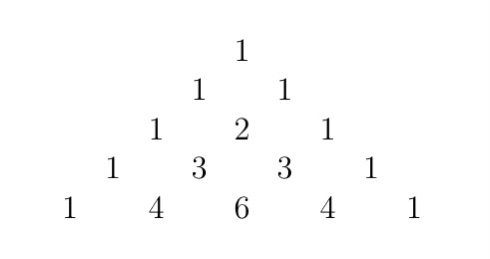
\includegraphics[scale=0.4]{./fig1/figure1.2.jpg}}


\begin{figure}
    \centering
$$\begin{array}{ccccccccccccc}
    & & & & 1 & & & & \\
    & & & 1 & & 1 & & & \\
    & & 1 & & 2 & & 1 & & \\
    & 1 & & 3 & & 3 & & 1 & \\
    1 & & 4 & & 6 & & 4 & & 1
\end{array}$$
    \caption{ 帕斯卡三角的0到4行}
\end{figure}


刚才给出的证明叫做\textsl{双射证明法}, 它是一种特别好的组合证明. 这是因为双射证明法可以将不同类型的组合对象联系起来, 有时会揭示出
意想不到的联系. 还要注意, 我们证明了$f$是双射是通过求它的逆, 而不是直接证明他是一对一的和映上的. 因为有一个$f^{-1}$的具体描述可以
在以后有用, 所以这是首选的方法. 最后, 在处理函数时, 我们总是从右向左去组合他们, 即
$$(f \circ g)(x)=f(g(x)).$$

现在我们通过他们的基数来计算子集. 对于集合$S$, 我们将使用如下符号
$$
\left(\begin{array}{l}
S \\ k
\end{array}\right)=\{T \subseteq S \mid \# T=k\}.
$$
例如,
$$
\left(\begin{array}{c}
\{a, b, c\} \\ 2
\end{array}\right)=\{\{a, b\},\{a, c\},\{b, c\}\}.
$$
正如预期的那样, 我们现在找到了这个集合的基数.
    \begin{thm}
    	\textsl{对}$n, k \geqslant 0$, 我们有
    		$$
    		\#\left(\begin{array}{c}
    		{[n]} \\ k
    		\end{array}\right)=\frac{n \downarrow_{k}}{k !}.
    		$$
    \end{thm}
    \begin{proof}
    	运用交叉相乘和定理1.2.1我们可知只需证明
    	$$
    	\# P([n], k)=k ! \cdot \#\left(\begin{array}{c}
    	{[n]} \\ k
    	\end{array}\right).
    	$$
    	为证上式, 我们可以取$\pi_{1} \ldots \pi_{k} \in P([n], k)$, 并且将其对应于子集$S=\left\{s_{1}, \ldots, s_{k}\right\} \subseteq[n]$,
    	并且对$S$以所有可能的情况进行排序. $S$的选取方法有$\#\left(\begin{array}{c}{[n]} \\ k\end{array}\right)$种, 再次由定理1.2.1, 排列
    	$S$中元素的方法有$k !$种. 由乘积法则即得结果. 证毕.
    \end{proof}


给定$n, k \geqslant 0$, 我们定义\textsl{二项式系数}如下
\begin{equation}
\left(\begin{array}{l}
n \\ k
\end{array}\right)=\#\left(\begin{array}{c}
{[n]} \\ k
\end{array}\right)=\frac{n \downarrow_{k}}{k !}.
\end{equation}
定义为这个名称的原因是这些数将出现在第三章研究的二项式展开中. 通常你会看到二项式系数显示在一个三角形数组中, 称为帕斯卡三角,
它的第$n$行的第$k$项是$\left(\begin{array}{l}n \\ k\end{array}\right)$, 当$k>n$时, 传统做法是省略0. 帕斯卡三角的0到4行见
图1.2. (很抱歉没有写出整个三角形, 但这一页不够大. )对$0 \leqslant k \leqslant n$, 我们可以用(1.3)来写
\begin{equation}
    \left(\begin{array}{l}
        n \\ k
        \end{array}\right)=\frac{n !}{k !(n-k) !}
\end{equation}
它的对称性令人愉悦. 我们也可以通过让$\left(\begin{array}{l}n \\ k\end{array}\right)=0$将二项式系数扩展到$k<0$. 在这种情况下,
它与$\left(\begin{array}{c}{[n]} \\ k\end{array}\right)=\varnothing$这一事实相符.

在下一定理中, 我们综合了有关二项式系数的各种基本结果, 这些结果在后面的定理中是有用的. 在这里, 我们会用到克罗内克函数, 定义如下
$$
\delta_{x, y}=\left\{\begin{array}{ll}
1 & \text { if } x=y, \\
0 & \text { if } x \neq y.
\end{array}\right.
$$
还要注意, 我们没有在(3)和(4)中指定求和变量$k$的范围, 因为它在更大的求和中额外的项都是0,
故它可以被视为$0 \leqslant k \leqslant n$或$k \in \mathbb{Z}$. 这两种观点都有用处.
    \begin{thm}
    	设$n \geqslant 0$.
    		(1)\ 对$n \geqslant 1$, 二项式系数满足初始条件
    		$$
    		\left(\begin{array}{l}
    		0 \\ k
    		\end{array}\right)=\delta_{k, 0}.
    		$$
    		和递推关系
    		$$
    		\left(\begin{array}{l}
    		n \\ k
    		\end{array}\right)=\left(\begin{array}{c}
    		n-1 \\ k-1
    		\end{array}\right)+\left(\begin{array}{c}
    		n-1 \\ k
    		\end{array}\right).
    		$$
    		(2)\ 二项式系数是对称的, 这意味着
    		$$
    		\left(\begin{array}{l}
    		n \\ k
    		\end{array}\right)=\left(\begin{array}{c}
    		n \\ n-k
    		\end{array}\right).
    		$$
    		(3)\ 我们有
    		$$
    		\sum_{k}\left(\begin{array}{l}
    		n \\ k
    		\end{array}\right)=2^{n}.
    		$$
    		(4)\ 我们有
    		$$
    		\sum_{k}(-1)^{k}\left(\begin{array}{l}
    		n \\ k
    		\end{array}\right)=\delta_{n, 0}.
    		$$
    \end{thm}
    \begin{proof}
    	(1)\ 初始条件是显然的. 对于递推关系, 设$\mathcal{S}_{1}$为集合$S \in\left(\begin{array}{c}{[n]} \\ k\end{array}\right)$, 其中$n \in S$,
    	设$\mathcal{S}_{2}$为集合$S \in\left(\begin{array}{c}{[n]} \\ k\end{array}\right)$, 其中$n \notin S$.
    	则$\left(\begin{array}{c}{[n]} \\ k\end{array}\right)=\mathcal{S}_{1} \uplus \mathcal{S}_{2}$. 但如果$n \in S$,
    	那么$S-\{n\} \in\left(\begin{array}{c}{[n-1]} \\ k-1\end{array}\right)$. 这就给出了一个$\mathcal{S}_{1}$与
    	$\left(\begin{array}{c}{[n-1]} \\ k-1\end{array}\right)$之间的双射, 于是$\# \mathcal{S}_{1}=\left(\begin{array}{c}n-1 \\ k-1\end{array}\right)$.
    	另一方面, 如果$n \notin S$, 那么$S \in\left(\begin{array}{c}{[n-1]} \\ k\end{array}\right)$, 这说明$\# \mathcal{S}_{2}=\left(\begin{array}{c}n-1 \\ k\end{array}\right)$
    	运用求和规则即得结论.

    	(2)\ 我们只需找到双射$f:\left(\begin{array}{c}{[n]} \\ k\end{array}\right) \rightarrow\left(\begin{array}{c}{[n]} \\ n-k\end{array}\right)$.
    	考虑映射$f:   2^{[n]} \rightarrow 2^{[n]}$, 且$f(S)=[n]-S$, 其中负号表示集合的差. 注意, 复合函数$f^{2}$是恒等映射, 因此$f$是一个双射,
    	此外, $S \in\left(\begin{array}{c}{[n]} \\ k\end{array}\right)$当且仅当$f(S) \in\left(\begin{array}{c}{[n]} \\ n-k\end{array}\right)$.
    	故$f$是被限制在这两个集合之间的双射.

    	(3)\ 对等式$$2^{[n]}=\biguplus_{k}\left(\begin{array}{c}{[n]} \\ k\end{array}\right)$$应用求和规则即得证.

    	(4)\ $n=0$的情况很简单, 所以我们设$n>0$. 我们将在下一章学习处理带符号方程的一般方法. 但现在我们试着证明等价的等式
    	$$
    	\sum_{k \text { 奇 }}\left(\begin{array}{l}
    	n \\ k
    	\end{array}\right)=\sum_{k \text { 偶 }}\left(\begin{array}{l}
    	n \\ k
    	\end{array}\right).
    	$$
    	设$\mathcal{T}_{1}$是$T \in 2^{[n]}$ 中 $\# T$为奇数的集合, $\mathcal{T}_{2}$是$T \in 2^{[n]}$ 中 $\# T$为偶数的集合.
    	我们希望找到一个双射$g: \mathcal{T}_{1} \rightarrow \mathcal{T}_{2}$. 考虑\textsl{对称差分}运算
    	$$
    	S \Delta T=(S-T) \uplus(T-S).
    	$$
    	不难看出$(S \Delta T) \Delta T=S$, 现我们用$g(T)=T \Delta\{n\}$定义$g: 2^{[n]} \rightarrow 2^{[n]}$. 因此, 由定义可得 $g^{2}$
    	是恒等映射. 此外$g$反转了奇偶性, 因此限制了所需的双射.
    \end{proof}


与排列和单词的情况一样, 我们希望枚举允许重复的“集合”. 一个\textsl{多重集}$M$是一个可以有重复的无序集合. 例如
$$
M=\left\{\left\{a^{3}, b, c^{2}\right\}\right\}.
$$
注意, 我们用双花括号表示多重集. 我们还将使用多重表示法, 其中$a^{m}$表示$m$个$a$相乘. 继续我们的例子
$$
M=\left\{\left\{a^{3}, b, c^{2}\right\}\right\}.
$$
与幂函数一样, 指数为1是可选的, 指数为0表示在这个多重集中没有这个元素. 多重集的\textsl{基数}是计算它的每个元素的重数和. 故
在我们的例子中$\# M=2+1+3=6$. 如果$S$是一个集合, 则$M$是$S$上的一个多重集, 如果$M$上的每个元素都是$S$中的一个元素.
我们令$\left(\left(\begin{array}{c}S \\ k\end{array}\right)\right)$是$S$上所有基数为$k$的多重集的集合, 且
$$
\left(\left(\begin{array}{l}
n \\ k
\end{array}\right)\right)=\#\left(\left(\begin{array}{c}
{[n]} \\ k
\end{array}\right)\right).
$$
例如
$$
\left(\left(\begin{array}{c}
\{a, b, c\} \\ 2
\end{array}\right)\right)=\{\{\{a, a\}\},\{\{a, b\}\},\{\{a, c\}\},\{\{b, b\}\},\{\{b, c\}\},\{\{c, c\}\}\}
$$
故$\left(\left(\begin{array}{l}3 \\ 2\end{array}\right)\right)=6$
   \begin{thm}
   	对$n, k \geqslant 0$我们有
   	$$
   	\left(\left(\begin{array}{l}
   	n \\ k
   	\end{array}\right)\right)=\left(\begin{array}{c}
   	n+k-1 \\ k
   	\end{array}\right).
   	$$
   \end{thm}
   \begin{proof}
   	我们希望找到一个双射
   	$$
   	f:\left(\left(\begin{array}{c}
   	{[n]} \\ k
   	\end{array}\right)\right) \rightarrow\left(\begin{array}{c}
   	{[n+k-1]} \\ k
   	\end{array}\right).
   	$$
   	给定一个在$[n]$上的多重集$M=\left\{\left\{m_{1} \leqslant m_{2} \leqslant m_{3} \leqslant \cdots \leqslant m_{k}\right\}\right\}$, 令
   	$$
   	f(M)=\left\{m_{1}<m_{2}+1<m_{3}+2<\cdots<m_{k}+k-1\right\}.
   	$$
   	现在$m_{i}+i-1$是不同的, 且由$m_{k} \leqslant n$有$m_{k}+k-1 \leqslant n+k-1$. 则$f(M) \in\left(\begin{array}{c}[n+k-1]) \\ k\end{array}\right)$
   	且这个映射是良好定义的. 现在读者可以很容易构造一个逆函数来证明$f$是一个双射.
   \end{proof}


和二项式系数一样, 我们把$\left(\left(\begin{array}{l}n \\ k\end{array}\right)\right)$扩展到负$k$并让他等于0.
以后我们会对其他自然定义域为$n, k \geqslant 0$的常数做同样地处理.

我们确实希望讨论计数集和多重集之间有一个有趣的关系. 注意, 定义(1.4)对于任何复数$n$都有良好定义, 因为下降的阶乘只是一个乘积, 同样
对于负整数也有意义. 事实上, 如果$n \in \mathbb{N}$, 则由定理1.3.4.
\begin{equation}
\left(\begin{array}{c}
-n \\ k
\end{array}\right)=\frac{(-n)(-n-1) \cdots(-n-k+1)}{k !}=(-1)^{k} \frac{n(n+1) \cdots(n+k-1)}{k !}=(-1)^{k}\left(\left(\begin{array}{l}
n \\ k
\end{array}\right)\right)
\end{equation}
在这种情况下, 一个枚举公式在负参数的计算下会产生另一个枚举函数, 称为组合互易, 我们将在3.9节中研究.

\section{集合划分}
我们已经知道不相交并是一个很好的组合性质. 故集合划分也扮演着重要角色就不足为奇了.

集合$T$的一个\textsl{划分}是集合$\rho$的非空子集$B_{1}, \ldots, B_{k}$使得$T=\uplus_{i} B_{i}$. 记作$\rho \vdash T$.
$B_{i}$被称为\textsl{块}, 我们用$\rho=B_{1} / \ldots / B_{k}$并去掉所有的花括号和逗号, 即使块的元素以及块本身是无序的.
例如, $T=\{a, b, c, d, e, f, g\}$的一个划分为
$$
\rho=a c f / b e / d / g=d / e b / g / c f a .
$$
我们令$B(T)$是所有$\rho \vdash T$的集合. 举个例子
$$
B(\{a, b, c\})=\{a / b / c, a b / c, a c / b, a / b c, a b c\}.
$$
第$n$贝尔数为$B(n)=\# B([n])$. 虽然$B(n)$没有已知的显示表达式, 但它有一个递归关系.
    \begin{thm}
    	贝尔数满足初始条件$B(0)=1$和递归关系, 即对$n \geqslant 1$有
    	$$
    	B(n)=\sum_{k}\left(\begin{array}{l}
    	n-1 \\ k-1
    	\end{array}\right) B(n-k)
    	$$
    \end{thm}

\begin{figure}
    \centering
$$\begin{array}{ccccccccccccc}
    & & & & 1 & & & & \\
    & & & 1 & & 1 & & & \\
    & & 1 & & 3 & & 1 & & \\
    & 1 & & 7 & & 6 & & 1 & \\
    1 & & 15 & & 25 & & 10 & & 1
\end{array}$$
    \caption{ 第二类斯特林数的1到5行}
\end{figure}

   \begin{proof}
   	初始条件即计算$\varnothing$的空划分. 对于递归, 给定$\rho \in B([n])$, 设$k$为包含$n$的分块$B$中元素的个数.
   	则有$\left(\begin{array}{l}n-1 \\ k-1\end{array}\right)$种方法在$[n-1]$中选取$B$中剩余的$k-1$个元素.
   	且划分$[n]-B$的方法有$B(n-k)$种. 把所有有可能的$k$求和即得证.
   \end{proof}


有时, 我们可能想要知道划分中分块的数量. 定义$S(T, k)$是所有含$k$个分块的$\rho \vdash T$的集合.

第二类斯特林数为$S(n, k)=\# S([n], k)$. 我们将在下一节介绍第一类斯特林数. 例如
$$
S(\{a, b, c\}, 2)=\{a b / c, a c / b, a / b c\}.
$$
故$S(3,2)=3$, 与二项式系数一样, $1 \leqslant k \leqslant n$ 时, $S(n, k)$可以用图1.3中的三角形表示, 且这些斯特林数满足一个简单的递推关系.
    \begin{thm}
    	贝尔数满足初始条件
    	$$S(0, k)=\delta_{k, 0},$$
    	且对$n \geqslant 1$有递归公式
    	$$
    	S(n, k)=S(n-1, k-1)+k S(n-1, k).
    	$$
    \end{thm}
    \begin{proof}
    	现在, 读者应该能毫不费力地证明初始条件了. 对于递归, $\rho \in S([n], k)$中的元素有两种:第一种, 删除$n$, 则剩下部分的拆分数量为$S([n-1], k-1)$,
    	这是一个双射. 这就解释了$S([n-1], k-1)$的和. 第二种, 删除$n$得到$\sigma \in S([n-1], k)$, 但这个映射不是双射. 特别地,
    	给定$\sigma$, 可以将$n$插入到它$k$块中的任一个以得到$S([n], k)$. 因此, 在这种情况下总计数是$k S(n-1, k)$.
    \end{proof}


\section{按圈结构排列}
将一个集合分解成一个拆分可以类比为将$[n]$的排列分解成圈. 这些是由第一类斯特林数来进行计数的.

\textsl{对称群}为$\mathfrak{S}_{n}=P([n])$. 顾名思义, $\mathfrak{S}_{n}$有一个定义如下的群结构. 如果$\pi=\pi_{1} \ldots \pi_{n} \in \mathfrak{S}_{n}$,
那么我们可以把这些排列看做一个双射$\pi:[n] \rightarrow[n]$, 其中$\pi(i)=\pi_{i}$. 由此可以得出$\mathfrak{S}_{n}$是一个用复合函数来计算的群.

给定$\pi \in \mathfrak{S}_{n}$, $i \in[n]$, 有一个最小的指数$\ell \geqslant 1$使得$\pi^{\ell}(i)=i$. 这和下面的各种其他声明将在1.9节中使用有向图
来证明. 在这种情况下, 元素$i, \pi(i), \pi^{2}(i), \ldots, \pi^{\ell-1}(i)$互不相同, 记
$$
c=\left(i, \pi(i), \pi^{2}(i), \ldots, \pi^{\ell-1}(i)\right)
$$
我们称它为长度为$\ell$的圈, 或简称为$\pi$的$\ell$-圈. 长度为1的圈称为\textsl{不动点}. 例如, 若$\pi=6514237$且$i=1$, 则
$\pi(1)=6, \pi^{2}(1)=3, \pi^{3}(1)=1$, 故$c=(1,6,3)$是$\pi$的一个圈. 现在我们重复这一过程:如果到目前为止还有$j \in[n]$
不存在于任一圈中, 那我们就找到包含$j$的圈使得每个元素都在一个圈中. $\pi$的\textsl{圈分解}是$\pi=c_{1} \ldots c_{k}$,
其中$c_{j}$是圈. 继续我们的例子可以得到
$$
\pi=(1,6,3)(2,5)(4)(7).
$$
为了将$\pi$的圈分解与其描述$\pi=\pi_{1} \ldots \pi_{n}$区别开, 我们称后者为$\pi$的单行表示法. 这也与两行表示法不同, 两行表示法是
一种写法如下
\begin{equation}
\pi=\begin{array}{cccc}
1 & 2 & \ldots & n \\
\pi_{1} & \pi_{2} & \ldots & \pi_{n}
\end{array}
\end{equation}
注意, 根据从哪个元素开始, $\ell$-圈有$\ell$种写法, 例如
$$
(1,6,3)=(6,3,1)=(3,1,6).
$$
此外, $\pi$的不同圈是不相交的. 所以如果我们把圈$c$看作$[n]$的排列, 它与$c$的元素一致并且所有其他元素都是不动点, 那么
$\pi=c_{1} \ldots c_{k}$的圈可交换由于我们认为乘积是排列的组合. 回到我们的例子, 我们可以写成
$$
\pi=(1,6,3)(2,5)(4)(7)=(4)(1,6,3)(7)(2,5)=(5,2)(3,1,6)(7)(4).
$$
如上所述, 我们将以下结果的证明推迟到1.9节.
  \begin{thm}
  	每个$\pi \in \mathfrak{S}_{n}$都有一个圈分解$\pi=c_{1} \ldots c_{k}$, 这个分解是唯一的且取决于因子的顺序和每个$c_{i}$
  	内元素的重新排序.
  \end{thm}
现在, 我们可以同时对上一节中给定数量块的集合划分进行研究. $n \geqslant 0$时, 我们用$c([n], k)$表示$\mathfrak{S}_{n}$
中具有$k$个圈的排列的集合. 注意表示圈数量的" $k$ 圈"与表示圈长度的" $k$ -圈"之间的区别. 第一类无符号的斯特林数是$c(n, k)=\# c([n], k)$.
故, 类似于我们之前看到的, 对$k<0$ 或$k>n$, 有$c(n, k)=0$. 为了理解这个符号
$$
c([4], 1)=\{(1,2,3,4),(1,2,4,3),(1,3,2,4),(1,3,4,2),(1,4,2,3),(1,4,3,2)\},
$$
故$c(4,1)=6$. 一般来说, 正如你在联系中需要证明的, $c([n], 1)=(n-1) !$. 第一类斯特林数的一部分展示在图1.4中. 同样, 我们有一个递归公式.
    \begin{thm}
    	第一类无符号斯特林数满足初始条件
    	$$
    	c(0, k)=\delta_{k, 0},
    	$$
    	且对$n \geqslant 1$有递归公式
    	$$
    	c(n, k)=c(n-1, k-1)+(n-1) c(n-1, k).
    	$$
    \end{thm}
    \begin{proof}
    	像往常一样, 我们关注递归公式. 给定$\pi \in c([n], k)$, 我们可以从他的圈中删除$n$. 若$n$是个不动点, 则结果为$c(n-1, k-1)$.
    	若$n$在一个长度至少为2的圈中, 则将$n$删除后我们得到的排列数为$c([n-1], k)$. 故我们必须找到$n$插入$\sigma \in c([n-1], k)$的方法数.
    	对于长度为$\ell$的圈, 有$\ell$个位置来插入$n$. 故可插入的位置为$\sigma$中所有圈的长度之和, 即$n-1$.
    \end{proof}

读者可能已经猜到, 还有一种(带符号的)第一类斯特林数定义如下:
$$
s(n, k)=(-1)^{n-k} c(n, k).
$$


\begin{figure}
    \centering
   $$\begin{array}{ccccccccccccc}
       & & & & 1 & & & & \\
       & & & 1 & & 1 & & & \\
       & & 2 & & 3 & & 1 & & \\
       & 6 & & 11 & & 6 & & 1 & \\
       24 & & 50 & & 35 & & 10 & & 1
   \end{array}$$
    \caption{  第一类斯特林数的1到5行}
\end{figure}



为什么要给这些常数加符号还不能马上看出来, 我们将在第五章了解到原因, 它表明$s(n, k)$是通过细化排序的分拆晶格的第一类惠特尼数.
在这里, 我们将用一个类比的方法来证明定理1.3.3的(4).
  \begin{cor}
  	对$n \geqslant 0$, 我们有
  	$$
  	\sum_{k} s(n, k)=\left\{\begin{array}{ll}
  	1 & \text { if } n=0 \text { or } 1, \\
  	0 & \text { if } n \geqslant 2.
  	\end{array}\right.
  	$$
  \end{cor}
   \begin{proof}
   	$n=0$或1的情况很容易验证, 故我们假设$n \geqslant 2 $. 因为$s(n, k)=(-1)^{n-k} c(n, k)$且 $(-1)^{n}$在整个求和过程中都是常数,
   	因此证明$\sum_{k}(-1)^{k} c(n, k)=0 $就够了. 利用定理1.5.2和对$n$进行归纳可得
   	$$
   	\begin{aligned}
   	\sum_{k}(-1)^{k} c(n, k) &=\sum_{k}(-1)^{k} c(n-1, k-1)+\sum_{k}(-1)^{k}(n-1) c(n-1, k) \\
   	&=-\sum_{k}(-1)^{k-1} c(n-1, k-1)+(n-1) \sum_{k}(-1)^{k} c(n-1, k) \\
   	&=-0+(n-1) 0 \\
   	&=0
   	\end{aligned}
   	$$
   	命题得证.
   \end{proof}

注意, 前面证明中考虑和的作用是除以$k \in \mathbb{Z}$而不是 $0 \leqslant k \leqslant n $. 这样就不用考虑$k=0$ 或 $k=n$
时的特殊情况了.

\section{整数分拆}
就像人们可以将一个集合划分成块一样, 一个非负整数也可以分割成一个和. 整数分拆不仅在组合学中占有重要地位, 而且在数论和对称群表示理论中也占有重要地位.
有关后者的更多信息, 请参阅附录A.

$n \geqslant 0$的\textsl{整数分拆}是一个正整数的多重集$\lambda$, $\lambda$的元素之和为$n$, 记为$\lambda \vdash n$ 或 $|\lambda|=n$.
其中, 令$|\lambda|=\sum_{i} \lambda_{i}$. 这些元素被称为部分. 由于$\lambda$的部分是无序的, 故我们通常按照规定顺序列出它们, 即弱减的$\lambda=\left(\lambda_{1}, \ldots, \lambda_{k}\right)$.
我们用$P(n)$表示$n$的所有分拆的集合, 且$p(n)=\# P(n)$. 例如,
$$
P(4)=\{(1,1,1,1),(2,1,1),(2,2),(3,1),(4)\}.
$$

\begin{figure}
    \centering
    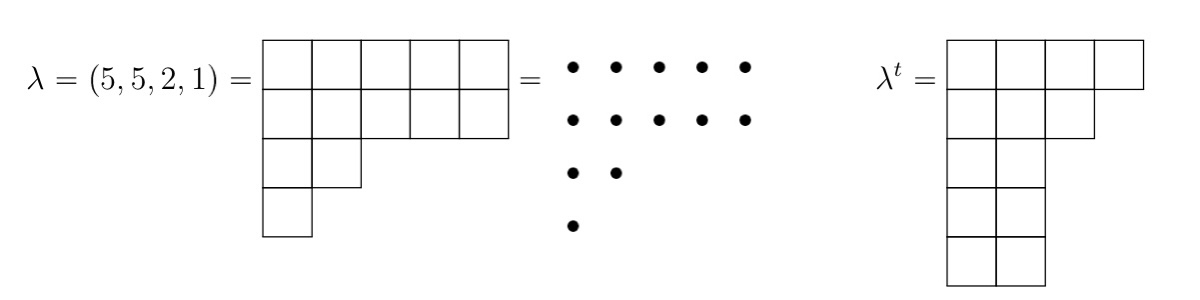
\includegraphics[scale=0.3]{./fig1/figure1.5.jpg}
    \caption{一个分拆, 它的杨图和共轭}
\end{figure}


\noindent 故$p(4)=5$. 注意$P([n])$与$P(n)$的区别, $P([n])$是集合划分的集合而$P(n)$是整数分拆的集合. 我们将对整数分拆使用多重表示法,
就像我们写多重集一样
$$
\lambda=\left(1^{m_{1}}, 2^{m_{2}}, \ldots, n^{m_{n}}\right)
$$
其中$m_{i}$为$i$在$\lambda$中的数量.

$p(n)$没有已知的闭式解. 事实上, 它甚至没有一个简单的递推公式. 人们可以用生成函数来得出这些数字的结果, 但这必须等到第三章.
这里我们只介绍一个有用的几何方法来研究$p(n)$. $\lambda=\left(\lambda_{1}, \ldots, \lambda_{k}\right) \vdash n$的\textsl{Ferrers}或杨图
为一个数组, 这个数组由$n$个左对齐的箱子组成, 其中第$i$行有$\lambda_{i}$个箱子. 有时我们也用点来代替箱子. 我们通常不将
分拆和它的杨图区分开来. $\lambda=(5,5,2,1)$的杨图如图1.5所示. 我们应该提醒读者, 我们用英文表示杨图, 其中行从1到$k$, 从上到下编号,
就像在一个矩阵中一样. 有些作者喜欢用法文表示, 在这种符号下, 行从下到上编号, 就像在笛卡尔坐标系中一样.
$\lambda$的\textsl{共轭}或\textsl{转置}是一个分拆$\lambda^{t}$, 这个分拆的杨图是通过关于$\lambda$的主对角线进行反射得到的.
这在图1.5中完成, 这表明$(5,5,2,1)^{t}=(4,3,2,2,2)$. 还有另一种方法来表示共轭的各部分.
  \begin{propo}
	若$\lambda=\left(\lambda_{1}, \ldots, \lambda_{k}\right)$是一个分拆且$\lambda^{t}=\left(\lambda_{1}^{t}, \ldots, \lambda_{l}^{t}\right)$, 则对$1 \leqslant j \leqslant l$,
	$$
	\lambda_{j}^{t}=\#\left\{i \mid \lambda_{i} \geqslant j\right\}.
	$$
   \end{propo}
   \begin{proof}
	由定义知, $\lambda_{j}^{t}$为$\lambda$第$j$列的长度. 但该列在第$i$行包含一个箱子当且仅当$\lambda_{i} \geqslant j$.
    \end{proof}

分拆$\lambda$的部分数称为它的长度, 记为$\ell(\lambda)$. 在这一点上, 读者可能希望讨论那些$\ell(\lambda)=k$的$n$的分拆.
其实, 考虑$P(n, k)$会更简单一些, 它是所有$n$的$\ell(\lambda) \leqslant k$的分拆的集合. 注意$\ell(\lambda)=k$的分拆$\lambda \vdash n$
的数量就是$p(n, k)-p(n, k-1)$. 所以在某种意义上这两种观点是等价的. 但是用$p(n, k)$来表示结果会更容易. 同时
$$
p(n, 0) \leqslant p(n, 1) \leqslant \cdots \leqslant p(n, n)=p(n, n+1)=\cdots=p(n)
$$
由于这种关系. 我们最好将$p(n, k)$表示在一个矩阵而不是一个三角形中, 记住, 第$n$行中的元素最终稳定为常数$p(n)$的无限重复.
这个数组的一部分将在图1.6中表示. 如果$n<0$ 或 $k<0$, 则令$p(n, k)=0$. 不像$p(n)$,  我们可以写出$p(n, k)$的一个简单的递归关系.
      \begin{thm}
     	$p(n, k)$满足
     	$$
     	p(0, k)=\left\{\begin{array}{ll}
     	0 & \text { 如果  }\,  k<0, \\
     	1 & \text { 如果  }\, k \geqslant 0,
     	\end{array}\right.
     	$$
     	和$n \geqslant 1$时,
     	$$
     	p(n, k)=p(n-k, k)+p(n, k-1)
     	$$
     \end{thm}

\begin{figure}
    \centering
    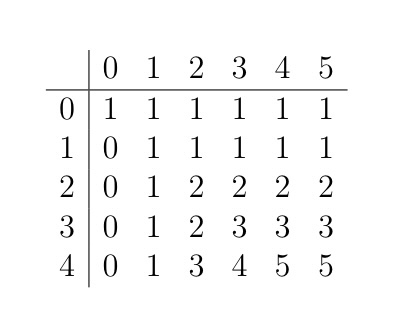
\includegraphics[scale=0.3]{./fig1/figure1.6.jpg}
    \caption{$0 \leqslant n \leqslant 4$, $0 \leqslant k \leqslant 5$时$p(n, k)$的值}
\end{figure}

    \begin{proof}
   我们直接跳到递归. 注意, 因为共轭是一个双射, $p(n, k)$也计算分拆$\lambda=\left(\lambda_{1}, \ldots, \lambda_{l}\right) \vdash n$, 其中$\lambda_{1} \leqslant k $.
   用$p(n, k)$的这种解释来证明会很方便. 我们有两种可能的情况. 若$\lambda_{1}=k$, 则$\mu=\left(\lambda_{2}, \ldots, \lambda_{l}\right) \vdash n-k$,
   且$\lambda_{2} \leqslant \lambda_{1}=k$. 故这个分拆可以用$p(n-k, k)$来计算. 另一种可能是$\lambda_{1} \leqslant k-1$. 这种情况可以用$p(n, k-1)$来计数.
   \end{proof}


\section{有序分拆}
回想一下, 整数分拆实际上是无序的, 即使我们通常以弱递减的方式列出它们. 这就引出了一个问题, 如果我们考虑把$n$写成和且有序会发生什么.
这就是有序分拆的概念.

$n$的\textsl{有序分拆}是一个正整数序列$\alpha=\left[\alpha_{1}, \ldots, \alpha_{k}\right]$, 称为部分且$\sum_{i} \alpha_{i}=n$.
我们记$\alpha \models n$, 并用方括号来区分有序分拆和整数分拆. 这导致$n$的有序分拆$[n]$与整数1到$n$之间出现符号冲突, 但
上下文应该清楚地表明这一点. 令$Q(n)$为所有$n$的有序分拆的集合且$q(n)=\# Q(n)$. 故4的有序分拆为
$$
Q(4)=\{[1,1,1,1],[2,1,1],[1,2,1],[1,1,2],[2,2],[3,1],[1,3],[4]\}.
$$
故$q(4)=8$, 即2的次幂. 正如作者喜欢说的那样, 这并非巧合.
      \begin{thm}
      	对$n \geqslant 1$我们有
      	$$
      	q(n)=2^{n-1} .
      	$$
      \end{thm}
     \begin{proof}
     	有一个著名的双射 $\phi: 2^{[n-1]} \rightarrow Q(n)$我们可以用来证明这个结果.
     	在第8章中使用准对称函数时这个映射将会很有用. 按递增顺序给定$S=\left\{s_{1}, \ldots, s_{k}\right\} \subseteq[n-1]$,
     	我们定义
     	\begin{equation}
     	\phi(S)=\left[s_{1}-s_{0}, s_{2}-s_{1}, \ldots, s_{k}-s_{k-1}, s_{k+1}-s_{k}\right]
     	\end{equation}
     	其中, 由定义, $s_{0}=0$且$s_{k+1}=n$. 为了表明$\phi$是良好定义的, 我们假设$\phi(S)=$ $\left[\alpha_{1}, \ldots, \alpha_{k+1}\right]$.
     	因为$S$是递增的, 故$\alpha_{i}=s_{i}-s_{i-1}$是一个正整数. 此外
     	$$
     	\sum_{i=1}^{k+1} \alpha_{i}=\sum_{i=1}^{k+1}\left(s_{i}-s_{i-1}\right)=s_{k+1}-s_{0}=n.
     	$$
     	因此$\phi(S) \in Q(n)$符合要求.

     	为了证明 $\phi$是双射, 我们构造它的逆$\phi^{-1}: Q(n) \rightarrow 2^{[n-1]}$. 给定$\alpha=$ $\left[\alpha_{1}, \ldots, \alpha_{k+1}\right] \in Q(n)$, 我们令
     	$$
     	\phi^{-1}(\alpha)=\left\{\alpha_{1}, \alpha_{1}+\alpha_{2}, \alpha_{1}+\alpha_{2}+\alpha_{3}, \ldots, \alpha_{1}+\alpha_{2}+\cdots+\alpha_{k}\right\}.
     	$$
     	读者应该不难证明$\phi^{-1}$是良好定义的且是$\phi $的倒数.
     \end{proof}

通常, 我们希望通过限制所讨论对象的组成部分的数目来作出更精确的计算. 设$Q(n, k)$为$n$的所有恰好有$k$个部分的有序分拆, 且$q(n, k)=\# Q(n, k)$.
由于$q(n, k)$将被证明是先前研究过的常数, 故我们不使用之前的三角. 通过前面的证明中限制函数$\phi$, 容易得出以下结果, 因此省略过程.
   \begin{thm}
   	有序分拆数满足
   	$$
   	q(0, k)=\delta_{k, 0}
   	$$
   	和
   	$$
   	q(n, k)=\left(\begin{array}{l}
   	n-1 \\
   	k-1
   	\end{array}\right).
   	$$
   	$n \geqslant 1$.
   \end{thm}

\section{十二模式}
现在我们已经有了计算特定函数的所有工具. 有12个这样的函数, 所以它们被称为十二模式, 这个概念是吉安-卡罗·罗塔在一系列讲座中介绍的.
这个名字是由乔尔·斯宾塞提出的, 不应该与佛教的十二重道相混淆!

我们将考虑三种类型的函数$f: D \rightarrow R$, 即任意函数, 单射和满射. 我们还允许定义域$D$和值域$R$各有两种类型:一种是
\textsl{可区分的}, 这意味着它是一个集合;一种是\textsl{不可区分的}, 这意味着它是一个由重复若干次的单个元素组成的多重集. 因此, 考虑的函数
总数为$f, D$和$R$所有可能数的乘积, 即$3 \cdot 2 \cdot 2=12 $. 我们将一直假设$|D|=n$ 及 $|R|=k$且它们都是非负整数.
我们将在图1.7的图表中整合结果.

首先, 如果$D$ 和 $R$都是可区分的. 在不丧失一般性的前提下, 我们可以假设$D=[n]$. 因此函数$f: D \rightarrow R$可以被看成一个单词
$w=f(1) f(2) \ldots f(n) $. 因为每个$f(i)$有$k$个选项. 根据定理1.2.2,这样的$f$ 有 $\# P(([k], n))=k^{n} $种. 如果$f$
是单射, 则$w$为一个排列, 由定理1.2.1可得有$\# P([k], n)=k \downarrow_{n}$ 种. 对于满射, 我们需要一个新的概念.
如果$D$是一个集合, 则函数$f: D \rightarrow R$的核是$D$的划分, 它的分块是$f^{-1}(r)$的非空子集, $r \in R $. 例如,
如果$f:\{a, b, c, d\} \rightarrow\{1,2,3\}$是由$f(a)=f(c)=2, f(b)=3$ 和 $f(d)=1$给出, 那么ker$ f = a c / b / d$.
如果$f$是满射, 那么函数可以通过选择$D$的一个划分指定ker $f$, 然后从ker $f$的分块到$R$选择一个双射$g$. 继续我们的例子,
$f$完全取决于其核与双射$g(a c)=2, g(b)=3$ 和 $g(d)=1$. 由定义, 选择 ker $f=B_{1} / \ldots / B_{k}$的方法有$S(n, k)$种.
利用单射下$n=k$的情况, 双射$g:\left\{B_{1}, \ldots, B_{k}\right\} \rightarrow R$的数量为$k \downarrow_{k}=k !$.
所以总数为$k ! S(n, k)$.

现在假设$D$是不可区分的, $R$是可区分的, 我们假设$R=[k]$. 那么可以认为$f: D \rightarrow R$是一个在$R$上的多重集
$M=\left\{\left\{1^{m_{1}}, \ldots, k^{m_{k}}\right\}\right\}$, 其中$m_{i}=$ $\# f^{-1}(i)$.
由此有 $\sum_{i} m_{i}=\# D=n $. 故根据定理1.3.4,这样的$f$数量为
$$
\left(\left(\begin{array}{l}
k \\ n
\end{array}\right)\right)=\left(\begin{array}{c}
n+k-1 \\ n
\end{array}\right)
$$


\begin{figure}
    \centering
    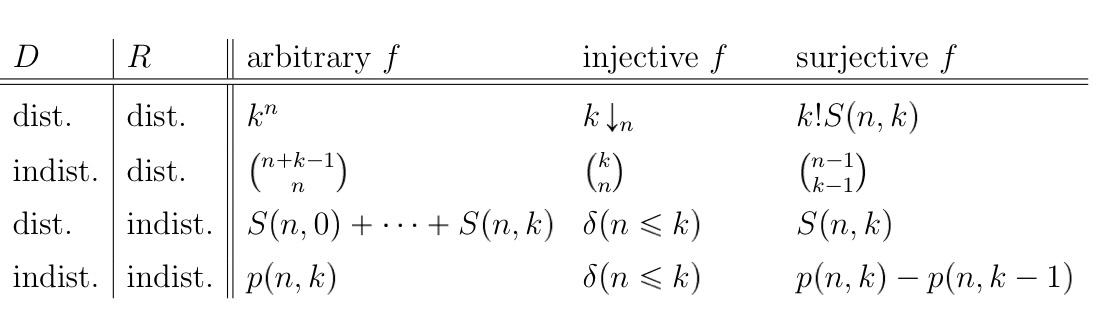
\includegraphics[scale=0.3]{./fig1/figure1.7.PNG}
    \caption{十二模式}
\end{figure}


\noindent
如果$f$为单射, 那么我们选择一个包含$n$个元素的$R=[k]$的子集, 其计数为$\left(\begin{array}{l}k \\ n\end{array}\right)$.
如果$f$是满射, 那么对所有$i$有$m_{i} \geqslant 1$, 故$\left[m_{1}, \ldots, m_{k}\right]$是$n$的一个有序分拆.
由定理1.7.2知, 这样的函数有$q(n, k)=\left(\begin{array}{c}n-1 \\ k-1\end{array}\right)$种.

为了处理$D=[n]$是可区分的而$R$是不可区分的情况, 我们引入克罗内克函数的一个有用扩展. 如果$S$是任一表述, 则
\begin{equation}
    \delta(S)=\left\{\begin{array}{ll}
        1 & \text { 若 }\  S \text{ 为真, } \\
        0 & \text { 若 } \ S \text{ 为假. }
        \end{array}\right.
\end{equation}
回到我们的计数, $f$完全由它的核决定, 也就是  $[n]$ 的一个划分. 如果我们考虑所有的$f$, 那么核可以有任意数量的分块直到包括$k$.
将相应的斯特林数相加得到图1.7中的相应结果. 如果$f$是单射, 那么为了这个函数存在, 必须有$n \leqslant k$. 在这种情况下,
只有一种可能的核, 即划分为单块. 这个计数为$\delta(n \leqslant k)$. 对于满射$f$, 我们将$[n]$划分为$k$个块, 这样就有$S(n, k)$种可能.

如果$D$ 和 $R$都是不可区分的, 那么对$r \in R$, $m_{i}=$ $\# f^{-1}(r)$的非零数完全决定了$f$. 这些数使得$n=\# D$至多划分成
$k=\# R$个部分. 回顾1.6节的符号, 这样的$f$总数为$p(n, k)$. 对于满射, 我们恰好需要$k$个部分, 故计数为$p(n, k)-p(n, k-1)$.

\section{图和有向图}
图论是组合学的重要组成部分. 我们将在后面利用有向图给出$\mathfrak{S}_{n}$中排列的圈分解存在唯一性的证明.

一个\textsl{标号图}$G=(V, E)$由一组称为\textsl{顶点}的元素$V$和一组称为\textsl{边}的元素$E$组成, 其中边由一对无序的顶点组成.
我们分别将$G$的顶点集和边集记为$V(G)$ 和 $E(G)$. 几何上, 我们认为顶点是节点, 而边是连接它们的线段或曲线.
通常, 图论中连接顶点$v$和$w$的边写成$e=v w$而不是$e=\{ v, w \}$. 这种情况下, 我们说$e$\textsl{包含}$v$和$w$,
或者说$e$有\textsl{端点}$v$和$w$, 我们也说$v$和$w$\textsl{相邻}. 例如, 图1.8中展示了图$G$, 它的顶点集为$V=\{v, w, x, y\}$,
边集为$E=\{v w, v x, v y, w x, x y\}$. 如果$\# V=1$, 则只有一个图有这样的顶点集, 我们把它叫做\textsl{平凡图}

如果$V(H) \subseteq V(G)$ 且 $E(H) \subseteq E(G) $, 则我们将图$H$称为图$G$的\textsl{子图}, 记为$H \subseteq G$.
在这种情况下, 我们也说$G$\textsl{包含}$H$. 接下来介绍几种重要的子图. 在图$G$中, 一个\textsl{长度为$\ell$的途径}是
一个顶点序列$W: v_{0}, v_{1}, \ldots, v_{\ell}$, 其中$v_{i-1} v_{i} \in E$, $1 \leqslant i \leqslant \ell $.
我们称这条途径为从\textsl{$v_{0}$ 到$v_{\ell},$}, 或称为一条\textsl{$v_{0}-v_{\ell}$途径}, 或称$v_{0}, v_{\ell}$是
$W$的\textsl{端点}. 如果所有顶点都是不同的, 则称$W$为路, 通常我们用字母$P$代表路. 特别地, 我们用 $W_{n}$ 或 $P_{n}$
来表示一条途径或一条有$n$个顶点的路径. 在我们的例图中, $P: y, v, x, w$是一条从$y$ 到 $w$长度为3的路. 注意, 长度指的是
路上的边的数量

\begin{figure}
    \centering
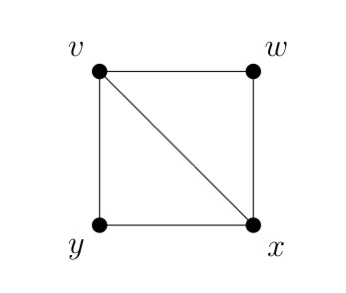
\includegraphics[scale=0.3]{./fig1/figure1.8.PNG}
    \caption{图$G$}
\end{figure}

\noindent
比顶点的数量少1. 在图$G$中, 一个\textsl{长度为$\ell$的圈}是顶点序列$C: v_{1}, v_{2}, \ldots, v_{\ell}$,
其中有互不相同的边$v_{i-1} v_{i}$, $1 \leqslant i \leqslant \ell$, 下标取$\ell$的模, 故 $v_{0}=v_{\ell}$.
在我们的例子中,  $C: v, x, y$是$G$中一个长度为3的圈. 在一个圈中, 长度即是顶点的数量也是边的数量. 我们用$C_{n}$表示一个
有$n$个顶点的圈, 我们称之为\textsl{$n$ -圈}. 我们用$K_{n}$表示\textsl{完全图}, 即包含$n$个顶点和它们之间所有可能的
$\left(\begin{array}{l}n \\ 2\end{array}\right)$ 条边. 我们刚才定义的图的某些部分之间有着密切的关系.
   \begin{lem}
   	设$G$是一个图,  $u, v \in V$
   	(1)\ 任意一条从$u$ 到 $v$的途径都包含一条从$u$ 到 $v$的路.
    (2)\ 任意两条不同的从$u$ 到 $v$的路的并集包含一个圈
   \end{lem}
     \begin{proof}
    	我们将证明(1), (2)作为练习. 令$W: v_{0}, \ldots, v_{\ell}$为一条途径, 对$\ell$进行归纳法,
    	即$W$的长度. 如果$\ell=0$, 则$W$就是条路. 故设$\ell \geqslant 1$. 如果$W$是条路, 则证毕. 如果不是, 那么$W$的顶点一定
    	有重复的, 记为$v_{i}=v_{j}$, $i<j$. 则我们有一条$u-v$途径$W^{\prime}: v_{0}, v_{1}, \ldots, v_{i}, v_{j+1}, v_{j+2}, \ldots, v_{\ell}$
    	比$W$更短. 由归纳法可知$W^{\prime}$包含路 $P$故$W$也包含 $P$.
    \end{proof}
设$\mathcal{G}(V)$是顶点集$V$上所有图的集合. 我们也将用$\mathcal{G}(V, k)$ 表示$\mathcal{G}(V)$中所有有$k$条边的图的集合.
      \begin{thm}
     	$n \geqslant 1$ ,  $k \geqslant 0$时我们有
     	$$
     	\# \mathcal{G}([n])=2^{\binom{n}{2}}
     	$$
     	及
     	$$
     	\# \mathcal{G}([n], k)=\left(\begin{array}{c}
     	\binom{n}{2} \\ k
     	\end{array}\right).
     	$$
     \end{thm}
     \begin{proof}
     	给定$V=[n]$, 则顶点集$V$的图$G$完全由其边集决定. 因为有$n$个顶点, 所以有$\binom{n}{2}$
     	种可能的边可供选择. 所以$\mathcal{G}([n])$中$G$的个数就是这些边的子集个数, 由定理1.3.1可知这种情况为2的次幂. 对于
     	$\mathcal{G}([n], k)$的证明是类似的, 只是使用了(1.4)的定义.
     \end{proof}

如果$V$中顶点不可区分, 则说它是未标号的. 如果图的类型从上下文来看比较清晰, 或对于目前做的事没有影响, 我们就省略形容词
“标号的”和“未标号的”. 未标号图的枚举比标号图复杂得多. 因此, 这个讨论被推迟到6.4节.

如果$G$是一个图且$v \in V$, 那么$v$的度为
$$
\operatorname{deg} v=  \text { 包含 } v \text{ 的 } e \in E \text { 的数量 }
$$
在我们的例子中,  $\operatorname{deg} v=\operatorname{deg} x=3$ ,  $\operatorname{deg} w=\operatorname{deg} y=2$.
顶点的度和边集的基数之间有很好的关系. 下一个结果说明了组合学中一种重要的证明方法:成对计数.

\begin{figure}
    \centering
    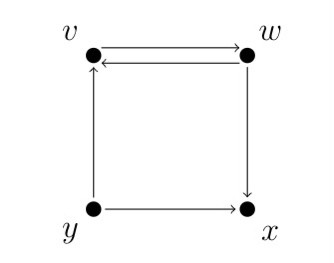
\includegraphics[scale=0.3]{./fig1/figure1.9.PNG}
    \caption{图$G$}
\end{figure}

     \begin{thm}
    	对任意图$G$有
    	$$
    	\sum_{v \in V} \operatorname{deg} v=2|E|.
    	$$
    \end{thm}
    \begin{proof}
    	考虑
    	$$
    	P=\{(v, e) \mid v \text {包含于} e\},
    	$$
    	则
    	$$
    	\# P=\sum_{v \in V}(\text { number of } e \text { containing } v)=\sum_{v \in V} \operatorname{deg} v.
    	$$
    	另一方面,
    	$$
    	\# P=\sum_{e \in E}(\text { number of } v \text { contained in } e)=\sum_{e \in E} 2=2|E|.
    	$$
    	将两种计数等同即证毕.
    \end{proof}

定理1.9.3通常被称为握手引理, 它有以下解释. 假设$V$是聚会上的一群人, 如果他们在庆祝活动中握手的话就在$v$和$w$之间画一条线.
然后把每个人握手的次数加起来, 为总共握手次数的两倍.

边的方向通常是有用的. 一个标号的有向图, 也叫有向图, 记为$D=(V, A)$, 其中$V$是顶点集而$A$是有序顶点对的弧集. 我们用
$a=\overrightarrow{v w}$表示弧, 并且说$a$\textsl{从$v$ 到$w$}. 例如, 图1.9中, 它有
$V=\{v, w, x, y\}$ 和 $A=\{\overrightarrow{v w}, \overrightarrow{w v}, \vec{w}, \overrightarrow{y v}, \vec{y}\}$.
我们用$V(D)$ 和 $A(D)$分别表示有向图$D$的顶点集和弧集. \textsl{有向途径}, \textsl{路}和\textsl{圈}的定义与无向的相似,
只是强调$i$在适当范围内有$\overrightarrow{v_{i-1} v_{i}} \in A$. 故, 在我们的例子中, $P: y, v, w, x$是有向路, $C: v, w$是有向圈.
注意,  $w, x, y, v$不是有向路, 因为$x$ 和 $y$ 之间的弧线方向错误.

令$\mathcal{D}(V)$ 和 $\mathcal{D}(V, k)$分别是有向图的集合与有$k$条弧的有向图的集合, 它们有顶点集$V$.
下一个结果的证明方式与定理1.9.2基本相同, 故省略.
     \begin{thm}
    	$n \geqslant 1$ ,  $k \geqslant 0$时有
    	$$
    	\# \mathcal{D}([n])=2^{n(n-1)}
    	$$
    	和
    	$$
    	\# \mathcal{D}([n], k)=\left(\begin{array}{c}
    	n(n-1) \\
    	k
    	\end{array}\right)
    	$$
    \end{thm}

在有向图$D$中有两种度. 顶点$v \in V$ 有\textsl{出度}和\textsl{入度}, 分别为
$$
\text{odeg }v= \text{满足} a=\overrightarrow{v w} \text{的} a \in A \text{的数量, }
$$
$$
\text{ideg} v= \text{满足} a=\overrightarrow{w v} \text{的} a \in A \text{的数量. }
$$
在图1.9中, odeg $v=1$ ,  ideg $v=2$. 下一个结果将允许我们完成1.5节剩下的证明. 有向图$D \cup E$的并集
是顶点集$V(D \cup E)=V(D) \cup V(E)$和弧集$\operatorname{arcs} A(D \cup E)=A(D) \cup A(E)$.
    \begin{lem}
   设$D=(V, A)$为有向图. 对于所有的$v \in V$有$v=\operatorname{ideg} v=1$当且仅当$D$是有向圈的不相交并集.
   \end{lem}
   \begin{proof}
   	反方向很容易看出, 因为$D$的任一顶点$v$的出度和入度都与包含$v$的有向圈中的度相同. 而在这样的圈中 odeg $ v=\operatorname{ideg} v=$1.
   \end{proof}

对于正向, 取任意$v=v_{1} \in V$. 因为odeg $v_{1}=1$ , 所以必然存在一个顶点$v_{2}$使得$\overrightarrow{v_{1} v_{2}} \in A $.
同理, 也必然存在$v_{3}$使得$\overrightarrow{v_{2}v_{3}} \in A$. 继续以这种方式生成序列$v_{1}, v_{2}, \ldots$,
由于$V$是有限的, 那么必有两个索引$i<j$使得$v_{i}=v_{j}$. 设$i$为最小的索引, $j$为$i$之后出现重复的第一个索引. 因此,
$i=1$, 因为如果不是, 那么我们有$\overrightarrow{v_{i-1} v_{i}}, \overrightarrow{v_{j-1} v_{i}} \in A$与
ideg $v_{i}=1$相矛盾. 由$j$的定义, 我们有一个有向圈$C: v_{1}, v_{2}, \ldots, v_{j-1}$. 此外, $C$的顶点不能卷入
另一条弧中, 否则会使它的出度和入度过大. 继续这样, 我们就可以把$D$分解成不相连的有向圈. \hfill\qedsymbol

有时, 允许图中边为$e=v v$的\textsl{环}是有用的. 同样, 我们可以允许有向图中的环为$a=\overrightarrow{v v}$.
另一种可能性是我们希望有\textsl{多条边}, 这意味着在给定的一对顶点之间可以有多条边, 这使得$E$成为一个多重集. \textsl{多个弧}的定义类似.
如果我们没有对我们的有向图做任何说明, 那么我们就假设它既没有圈也没有多条边. 现在我们来证明定理1.5.1.

\textsl{定理1.5.1的证明}. 对任意$\pi \in \mathfrak{S}_{n}$, 我们将其与包含$V=[n]$和弧$\overrightarrow{ij} \in A$
(等价于$\pi(i)=j$)的函数有向图$D_{\pi}$联系起来. $D_{\pi}$是一个有环的有向图. 因为 $\pi$ 是一个函数, 且对所有$i \in[n]$
有odeg $i=1$. 而且因为 $\pi$ 是双射, 故对所有$i$有ideg $i=1$. 如果允许环存在, 前面引理的证明同样有效. 故$D_{\pi}$
是圈的不相交并. 但有向图$D_{\pi}$的圈对应的是排列的圈. 因此存在$\pi$的圈分解. 在引理1.9.5的必要性论证中,
也很容易验证这样分解产生的$D_{\pi}$的圈是否唯一. 这意味着关于圈的唯一性命题我们做完了. \hfill\qedsymbol

\section{树}
树是一种图, 它经常出现在实践中, 甚至出现在数学之外的领域. 例如, 树在计算机科学中用作数据结构, 或在遗传学中用作进化模型.
如果每一对顶点$v, w \in V$ 都存在一条$G$中的途径从$v$到$w$, 则称$G$是\textsl{连通的}. 由引理1.9.1的(1), 这相当于存在
$G$中的一条从$v$到$w$的路. $G$的\textsl{连通部分}是最大连通子图. 如果$G$连通, 则只有一个部分. 如果$G$中没有圈, 则称
它为\textsl{无圈的}. 无圈图的另一个名称为\textsl{森林}. 森林的连通部分称为\textsl{树}. 故, 如果图$T$连通且无圈,
那么它就是树. 图1.10包含五棵树$T_{1}, \ldots, T_{5}$.

图$G$的\textsl{叶子}是deg$ v=1$ 的顶点$v$. 下一个结果将显示非平凡的树有叶子(不管一年中的什么时候). 此外, 从这个引理可以
清楚地看出, 为什么叶子是树的一个有用的归纳工具. 为了说明, 我们需要下面的符号. 如果$G$是一个图且$W \subseteq V$, 则
图$G-W$的顶点集为$V-W$, 边集由$E$中所有端点在$V-W$中的边组成. 如果对某些$v$有$W=\{v\}$, 那么我们把$G-\{v\}$记为$G-v$.
在图1.10中, $T_{2}=T_{1}-5$. 同理, 如果$F \subseteq E$ , 那么图$G-F$的顶点集为 $V(G-F)=V(G)$ , 边集为 $E(G-F)=E(G)-E(F)$
如果$F$只有一条边, 那么我们我们使用与顶点类似的缩写.
          \begin{lem}
         	设$T$是一棵$\# V \geqslant 2$的树
            (1)\ $T$至少有两片叶子.
            (2)\ 如果$v$是$T$的叶子, 那么$T^{\prime}=T-v$也是一棵树.
         \end{lem}

\begin{figure}
    \centering
    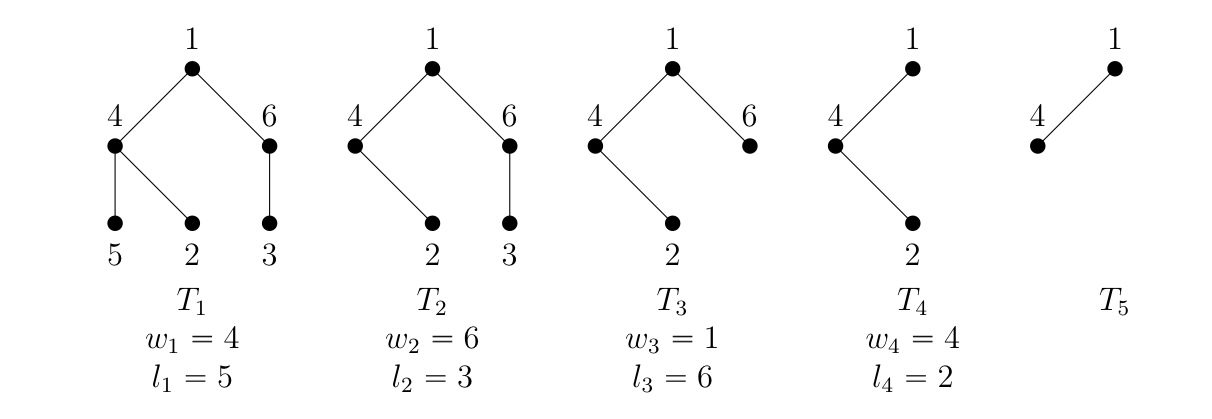
\includegraphics[scale=0.3]{./fig1/figure1.10.PNG}
    \caption{Prüfer算法}
\end{figure}
    \begin{proof}
   	(1)设 $P: v_{0}, \ldots, v_{\ell}$ 是$T$中最长的一条路. 因为$T$是非平凡的, $v_{0} \neq v_{\ell}$.
   	可证$v_{0}, v_{\ell}$是叶子, 我们将证明$v_{0}$, 同样地证明也适用于$v_{\ell}$. 假设 deg$v_{0} \geqslant 2$. 那么一定
   	有一个顶点$w \neq v_{1}$使得$v_{0} w \in E$. 现在有两种可能. 如果$w$不是$P$的顶点, 则$P^{\prime}: w, v_{0}, \ldots, v_{\ell}$
   	比$P$更长, 与$P$的定义相矛盾. 如果$w=v_{i}$, $2 \leqslant i \leqslant \ell$, 则$P$从$v_{0}$ 到 $v_{i}$连同边$v_{0} v_{i}$
   	形成了$T$中的一个圈, 再次矛盾.

   	(2) 显然 $T^{\prime}$是无圈的, 因为移除顶点不能创建一个圈. 为了证明它是连通的, 取$x, y \in V\left(T^{\prime}\right)$.
   	因为$T$是连通的, 故$x, y$也是$T$的顶点. 引理1.9.1的(1)表明$T$中有一条从$x$到$y$的路$P$. 如果这条路也在 $T^{\prime}$中,
   	则证明完成. 但如果$P$经过$V$, 那么, 因为只有一个唯一的顶点$v^{\prime}$与$v$相邻, 所以$P$在经过$v$之前与之后都必须经过
   	$v^{\prime}$. 这就与$P$的所有顶点都是不同的相矛盾.
   \end{proof}

树有许多特征. 我们在这里收集了一些, 因为它们在后续中有用.
      \begin{lem}
     	设$T$是$\# V=n$ 及 $\# E=m$的图. 下面是$T$为树的等价条件.

     	\noindent(1) $T$是连通的且无圈.

     	\noindent(2) $T$是无圈的且$n=m+1$.

        \noindent(3) $T$是连通的且$n=m+1$.

     	\noindent(4) 对于每一对顶点$u, v$, 都有一条唯一的从$u$到$v$路径.
     \end{lem}
     \begin{proof}
     	我们将证明(1),(2),(3)的等价性. (1)与(4)的等价性留作练习. 要证明(1)可推(2),通过归纳法证明
     	$n=m+1$就够了.  $n=1$时易证, 如果 $n \geqslant 2$, 由引理1.10.1, $T$有一个叶子$v$. 对$T^{\prime}=T-v$, 它的顶点数
     	与边数的关系为$n^{\prime}=m^{\prime}+1$. 但$n=n^{\prime}+1$ 且 $m=m^{\prime}+1$ , 故$n=m+1$.

     	要证(2)可推(3), 考虑$T$的连通部分$T_{1}, \ldots, T_{k}$. 因为$T$是无圈的, 所以每个连通部分都是树. 由
     	(1) $\Longrightarrow$ (2), 我们有$n_{i}=m_{i}+1$, $1 \leqslant i \leqslant k$, 其中 $n_{i}=\# V\left(T_{i}\right)$ 且
     	$m_{i}=\# E\left(T_{i}\right)$. 因为有$\sum_{i} n_{i}=n$ 及 $\sum_{i} m_{i}=m$, 故把这些等式加在一起可得$n=m+k$.
     	又因为$n=m+1$, 故$k=1$. 这意味着$T$只有一个部分, 故是连通的.

     	我们用反证法由(3)推(1). 假设$T$包含一个圈$C$, 令$e=u v \in E(C)$. 我们说$T-e$仍是连通的. 如果$x, y$是$T-e$中任意两个顶点,
     	那么在$T$中有一个从$x$ 到 $y$的途径$W$. 如果$W$不包含$e$, 那么$W$仍在$T-e$中. 如果$W$包含$e$, 则将$W$中的$e$替换为
     	路$C-e$, 形成$T-e$中从$x$到$y$的新途径$W^{\prime}$. 我们可以一直这样移除边直到得到的图$T^{\prime}$是无圈的, 因为
     	$T^{\prime}$仍然是连通的, 所以它是一棵树, 故$n^{\prime}=m^{\prime}+1 $, 但$n^{\prime}=n$ 且 $m^{\prime}<m$
     	所以$n<m+1$, 矛盾. \hfill\qedsymbol

     	设$\mathcal{T}(V)$是顶点集$V$上所有树的集合. 对于$\# \mathcal{T}(V)$, 下面这个漂亮的公式有很多不同的证明, 其中很多
     	在Moon的书中都有.
     \end{proof}
    \begin{thm}
   	当$n \geqslant 1$时, 我们有
   	$$
   	\# \mathcal{T}([n])=n^{n-2}.
   	$$
   \end{thm}
   \begin{proof}
   	$n=1$的情况易证, 所以假设$n \geqslant 2$. 由定理1.2.2可以找到一个双射$f: \mathcal{T}([n]) \rightarrow P(([n], n-2))$.
   	有一个著名的构造$f$的算法叫做\textsl{Prüfer算法}, 图1.10为示例. 给定$T \in \mathcal{T}([n])$, 为了求$f(T)=w_{1} \ldots w_{n-2}$,
   	我们构造一个通过将$T$的顶点移除的树的序列$T=T_{1}, T_{2}, \ldots, T_{n-1}$, 如下所示, 由于$T$的顶点标记为$1, \ldots, n$,
   	所以我们可以找到最大顶点. 给定$T_{i}$, 我们找到叶子$l_{i} \in V\left(T_{i}\right)$使得$l_{i}$最大, 并且令 $T_{i+1}=T_{i}-l_{i}$.
   	由先前的引理, $T_{i+1}$也是一棵树. 因为$l_{i}$是叶子, 故它只与$T_{i}$中的$w_{i}$相邻, 其中$w_{i}$是$f(T)$中的第$i$个元素.
   	现根据定义, 每个$w_{i} \in[n]$ 与 $f(T)$长度为 $n-2$. 故$f(T) \in P(([n], n-2))$.

   	为了证明$f$是双射, 我们要找到它的逆. 给定$w \in P(([n], n-2))$ , 我们首先构造一个排列$l=l_{1} \ldots l_{n-2} \in P([n], n-2)$ ,
   	其中$l_{i}$是从$T_{i}$中移除的叶子, 将$T_{i}$移除$l_{i}$后得到$T_{i+1}$. 故我们构造$l_{i}$为
   	\begin{equation}
   	l_{i}=\max \left([n]-\left\{l_{1}, \ldots, l_{i-1}, w_{i}, \ldots, w_{n-2}\right\}\right)
   	\end{equation}
   	最后我们构造$f^{-1}(w)=T$, 这里$T$的边为$e_{i}=l_{i} w_{i}$, $1 \leqslant i \leqslant n-2$, 以及边$e_{n-1}=l_{n-1} l_{n}$, 其中
   	$[n]-\left\{l_{1}, \ldots, l_{n-2}\right\}=\left\{l_{n-1}, l_{n}\right\} $ . 为了证明$f^{-1}(w)=T$是树, 首先注意
   	$l_{1}$是$T$的叶子, 因为由(1.10)和$e_{n-1}$的定义, $l_{1}$与$w_{1}$相邻且不与$T$的其他任何叶子相邻. 考虑$w^{\prime}=w_{2} \ldots w_{n-2}$ ,
   	用集合$[n]-\left\{l_{1}\right\}$ 代替 $[n]$来将算法$f^{-1}$ 应用到 $w^{\prime}$上. 通过归纳, 得到树$T^{\prime}$.
   	而$T$是通过把$l_{1}$作为叶子加到$T^{\prime}$上形成的, 故$T$也是一棵树.

   	为了证明$f$ 和 $f^{-1}$互逆, 我们将证$f^{-1} \circ f$ 是恒等映射, 将$f \circ f^{-1}$的证明留给读者. 设 $f(T)=w_{1} \ldots w_{n-2}$,
   	同时, 令在构造$f(T)$时移除的叶子序列为$l_{1}^{\prime} \ldots l_{n-2}^{\prime}$. 那么根据算法的定义, $T$的边为
   	$l_{i}^{\prime} w_{i}$ ,  $1 \leqslant i \leqslant n-2$, 以及$l_{n-1}^{\prime} l_{n}^{\prime}$ ,
   	其中 $[n]-\left\{l_{1}^{\prime}, \ldots, l_{n-2}^{\prime}\right\}=\left\{l_{n-1}^{\prime}, l_{n}^{\prime}\right\}$.
   	将它与$f^{-1}$的定义比较我们可证对所有$i$有$l_{i}=l_{i}^{\prime}$, 且如果我们能证明对$1 \leqslant i \leqslant n-2$等式成立
   	则证明完成. 因为$l_{i}^{\prime}$是$T_{i}$中一个叶子, 所以它不能是之前被移除的叶子$l_{1}^{\prime}, \ldots, l_{i-1}^{\prime}$.
   	其余的顶点中, $w_{i}, \ldots, w_{n-2}$不是这个叶子, 因为它们与将要被移除的叶子相邻. 相反, 那些不属于$w_{i}, \ldots, w_{n-2}$
   	的必须是叶子, 否则只要它们相邻的叶子被移除就会被列为 $w_{j}$, $j \geqslant i$. 因此$T_{i}$的叶子一定是
   	$[n]-\left\{l_{1}^{\prime}, \ldots, l_{i-1}^{\prime}, w_{i}, \ldots, w_{n-2}\right\}$ 中的元素.
   	因为我们总是移除最大的叶子, 所以我们可以得到选择 $l_{i}^{\prime}$与(1.10)的方法完全相同. 因此$l_{i}=l_{i}^{\prime}$得证.
   \end{proof}


\section{格路}
格路可以引出组合学中许多有趣的问题. 它们在概率与统计中也很重要;参见Mohanty的书.

考虑平面上的\textsl{整数格}
$$
\mathbb{Z}^{2}=\{(x, y) \mid x, y \in \mathbb{Z}\}.
$$
\textsl{格路}是由$\mathbb{Z}^{2}$上的元素 $P:\left(x_{0}, y_{0}\right),\left(x_{1}, y_{1}\right), \ldots,\left(x_{\ell}, y_{\ell}\right) $
组成的序列. 与图论中一样, 我们说路从$\left(x_{0}, y_{0}\right)$ 到 $\left(x_{\ell}, y_{\ell}\right)$有\textsl{长度}$\ell$,
$\left(x_{0}, y_{0}\right)$ 与 $\left(x_{\ell}, y_{\ell}\right)$是它的端点. 与图论的路不通, 我们不假定$\left(x_{i}, y_{i}\right)$是不同的.
为了说明这个符号, 如果我们假设图1.11中左边的路从原点开始, 那么它将被写成
$$
P:(0,0),(0,1),(0,2),(1,2),(1,3),(2,3),(3,3),(3,4),(4,4).
$$
$P$上$\left(x_{i-1}, y_{i-1}\right)$ 和 $\left(x_{i}, y_{i}\right)$之间的\textsl{步}是向量$s_{i}=\left[x_{i}-x_{i-1}, y_{i}-y_{i-1}\right]$.
注意使用方括号和圆括号来区分步与路中的顶点. 注意$P$是由它的步决定的, 且完全由它的步和初始顶点决定. 如果没有指


\begin{figure}
    \centering
    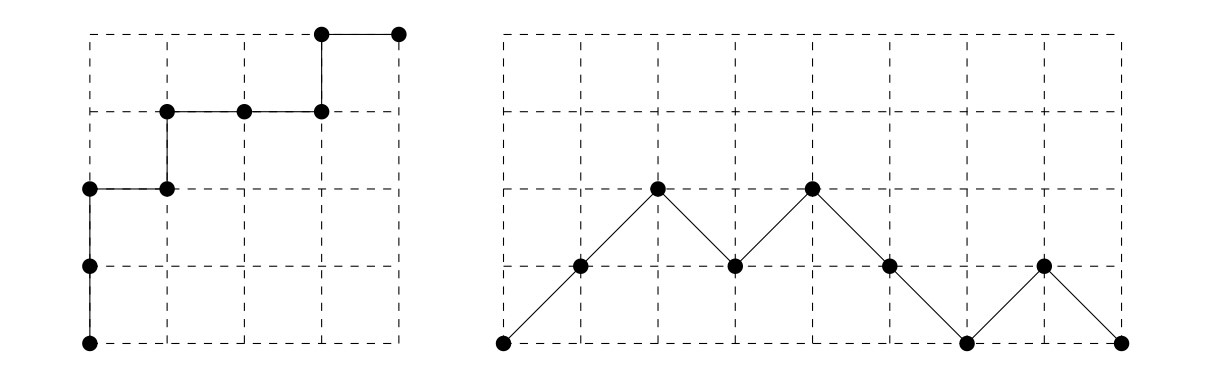
\includegraphics[scale=0.3]{./fig1/figure1.11.PNG}
    \caption{Dyck路}
\end{figure}


\noindent
定初始顶点, 则设它是原点. 设$E=[1,0]$ 与 $N=[0,1]$分别为\textsl{向东}和\textsl{向北}步. 图1.11左边的路也可表示为$P: N N E N E E N E$.

我们用符号 $\mathcal{N} \mathcal{E}(m, n)$表示从 (0,0) 到 $(m, n)$的格路, 且只使用向东步和向北步. 我们称只使用$N$和$E$步的格路为\textsl{东北路}.
       \begin{thm}
      	$m, n \geqslant 0$时, 有
      	$$
      	\# \mathcal{N} \mathcal{E}(m, n)=\left(\begin{array}{c}
      	m+n \\
      	m
      	\end{array}\right)
      	$$
      \end{thm}
      \begin{proof}
      	设$P$是从(0,0) 到 $(m, n)$的东北路, 则$P$共有$m+n$步. 且一旦有$m$步选为$E$, 则其余的必然是$N$.
      \end{proof}
我们将关注一种特殊的东北路. 一条从$(0,0)$开始,  到 $(n, n),$ 结束, 且从不低于直线$y=x$的东北路称为\textsl{半长为$n$的Dyck路}.
图1.11中的第一条路就是这种类型的. 注意, $n$被称为半长是因为Dyck路本身有$2n$步. 我们用$\mathcal{D}(n)$表示半长为$n$的Dyck路的集合.
这不会与顶点集$V$上的有向图$\mathcal{D}(V)$混淆, 因为前者的符号$n$是一个非负整数而后者是一个集合. 我们现在定义\textsl{卡特兰数}如下
$$
C(n)=\# \mathcal{D}(n)
$$
卡特兰数在组合学中随处可见. 事实上, Stanley写了一本书, 其中包含214种不同的$C(n) $的组合解释.
       \begin{thm}
      	我们有初始条件
      	$$
      	C(0)=1
      	$$
      	和$n \geqslant 1$时的递归关系
      	$$
      	C(n)=C(0) C(n-1)+C(1) C(n-2)+C(2) C(n-3)+\cdots+C(n-1) C(0)
      	$$
      \end{thm}
      \begin{proof}
      	初始条件计算的是只有一个顶点的路. 对于递归, 取$P: v_{0}, \ldots, v_{2 n} \in \mathcal{D}(n)$, 其中
      	对所有$i$有$v_{i}=\left(x_{i}, y_{i}\right)$. 设$j>0$是使得 $v_{2 j}$在直线 $y=x$上最小的下标. 因为$v_{2 n}=(n, n)$
      	满足这个条件, 所以这样的指标一定存在. 还要注意, 在$y=x$上没有奇数下标的顶点, 因为在该顶点之前的向北步与向东步地步数不可能相等.
      	故我们可得 $P_{1}$, 即从$v_{1}$ 到 $v_{2 j-1}$的部分, 它保持在$y=x+1$之上. 所以可选择的$P_{1}$有$C(j-1)$种.
      	如果$P_{2}$是$P$从$v_{2 j}$ 到 $v_{2 n}$的一部分, 则$P_{2}$是半长为$n-j$的Dyck路. 故可选择的$P_{2}$有$C(n-j)$种.
      	因此所有这样的$P$有$C(j-1) C(n-j)$种, 再把所有$1 \leqslant j \leqslant n$ 相加即证毕.
      \end{proof}

卡特兰数有一个显示表达式, 但为了推导这个公式, 我们使���由$C(n)$计算的第二种路更为方便. 我们分别称$U=[1,1]$ 与 $D=[1,-1]$
\textsl{升步}和\textsl{降步}. 则\textsl{升降路}为只使用升步与降步的路. 显然, 如果我们令$\tilde{\mathcal{D}}(n)$
为不低于$x$轴的从(0,0)到$(2 n, 0)$ 的升降路的集合, 则$\# \tilde{\mathcal{D}}(n)=\# \mathcal{D}(n)=C(n)$. 事实上,
通过旋转和平面膨胀可以从一个集合的路对应到另一个平面的路. 图1.11中的两条路在这个映射下对应, 第二条路径表示为$P: U U D U D D U D$.
     \begin{thm}
    	$n \geqslant 0$时有
    	$$
    	C(n)=\frac{1}{n+1}\left(\begin{array}{c}
    	2 n \\ n
    	\end{array}\right).
    	$$
    \end{thm}
    \begin{proof}
    	我们把右边改写为
    	$$
    	\frac{1}{n+1}\left(\begin{array}{c}
    	2 n \\ n
    	\end{array}\right)=\frac{(2 n) !}{n !(n+1) !}=\frac{1}{2 n+1}\left(\begin{array}{c}
    	2 n+1 \\ n
    	\end{array}\right).
    	$$
    	设$\mathcal{P}$为从(0,0)开始到 $(2 n+1,-1)$结束的所有升降路的集合, 这样的路有$2 n+1$步, 其中$n$步是升的(这使得其他$n+1$步是降的),
    	故$\# \mathcal{P}=\left(\begin{array}{c}2 n+1 \\ n\end{array}\right)$. 我们需要找到$P$的一个划分$\rho$满足以下条件:

    	1. $\rho$的每个分块$B$都有$\# B=2 n+1$

    	2. $\rho$的分块与 $\tilde{\mathcal{D}}(n)$中的路之间存在双射.

    	\noindent
    	这可得到$\# \tilde{\mathcal{D}}(n)$ 等于$\rho$ 的分块数, 即$\# \mathcal{P} /(2 n+1)$, 从而得到需要的等式.

    	为了确定$\rho$, 我们取任意 $P \in \mathcal{P}$ 并说分块$B$包含$P$. 我们将$P$的顶点$v$的$y$坐标称为它的\textsl{高度}, 记为ht $v$.
    	假设$P$可由步表示为$P: s_{1} s_{2} \ldots s_{2 n+1}$. 定义$P$的第$r$次旋转为路
    	$$
    	P_{r}: s_{r+1} s_{r+2} \ldots s_{2 n+1} s_{1} s_{2} \ldots s_{r}
    	$$
    	其中, 所有路都从原点开始. 令$B=\left\{P_{0}, \ldots, P_{2 n}\right\}$. 为了证明$B$有正确的基数, 我们必须证明$P_{i}$
    	是不同的. 假设存在两条路是相等的, 我们可以重新编号, 使得存在$1 \leqslant j \leqslant 2 n$有$P_{0}=P_{j}$.
    	取$j$为最小的一个. 迭代这个等式, 我们可以得到 $P_{0}=P_{j}=P_{2 j}=\ldots$这些等式, 以及$j$越小越好, 这意味着
    	$P=P_{0}$连接了$P^{\prime}: s_{1} \ldots s_{j}$与它自身, 且$P$为它的$k$倍, $k \geqslant 2$. 设$P^{\prime}$在高度为$h$时结束, 那么$P$必须在高度为$kh$时结束,
    	因此$k h=-1$. 这就使得$k=1$, 矛盾.

    	为了完成证明, 我们必须证明$\rho$的分块与$\tilde{\mathcal{D}}(n)$中的路是双射的. 设$\tilde{\mathcal{D}}^{\prime}(n)$
    	为在$\tilde{\mathcal{D}}(n)$中的每条路再加上一个降步所得到的路的集合. 故$\rho$的划分$\mathcal{P} \supseteq \tilde{\mathcal{D}}^{\prime}(n)$.
    	这就足以说明在$\rho$的每一个分块$B$都有唯一一条$\tilde{\mathcal{D}}^{\prime}(n)$中的路. 令$B$像前一段那样旋转路生成的,
    	设$P: v_{0} \ldots v_{2 n+1}$为$P$的格点, $h$是$P$的一个顶点的最小高度, 然后在$P$中所有高度为$h$的顶点中设$v_{r}$为最左边的那个.
    	我们说$P_{r} \in \tilde{\mathcal{D}}^{\prime}(n)$且对$s \in\{0,1, \ldots, n\}-\{r\}$没有其他的$P_{s}$在这个集合中.
    	我们将证明这两个声明中的第一个. 由于 $v_{r}$被移到了原点, 且在$P$中高度最小, 所以$i \geqslant r$时其他所有$v_{i}$平移后
    	都保持在$x$轴上方. 至于$i<r$时的$v_{i}$, 他们也必须被平移, 因此$v_{r}$是$P_{r}$的最后一个顶点, 且高度为$-1 $. 但由于
    	$v_{r}$ 是$P$中第一个高度最小的顶点, 在它之前的所有顶点的高度一定比它大, 即大于$-1$, 因此它们也必须在$x$轴上方(或之上).
    	因此只有$P$的最后一个顶点在$x$轴下方, 这就是我们想要证明的.
    \end{proof}

\section{有禁模式}
有禁模式是组合学中一个相对较新的研究领域. 由于它与代数几何和计算机科学的联系, 它有了很多的发展, 有关此主题的更多信息请参阅Bóna或Kitaev的书.

\begin{figure}
    \centering
    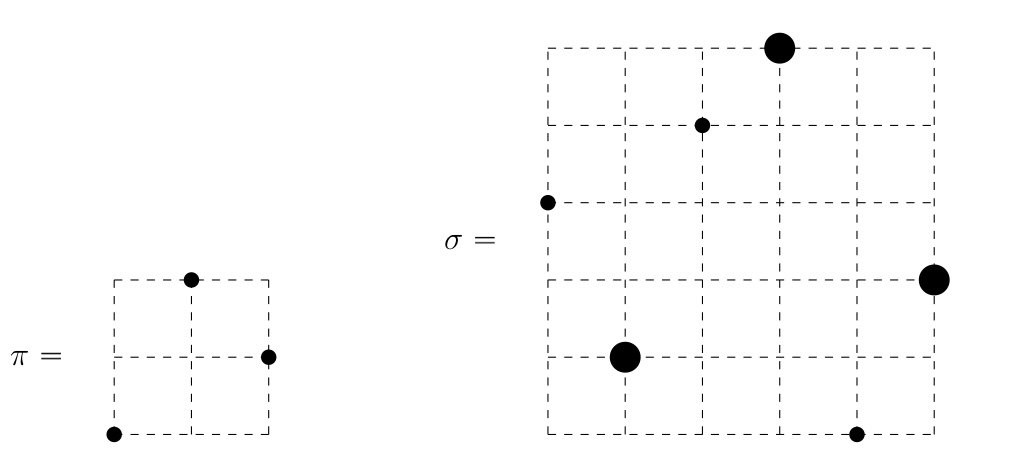
\includegraphics[scale=0.3]{./fig1/figure1.12.PNG}
    \caption{$\pi=132$与$\sigma=425613$}
\end{figure}


设$S$是$\# S=k$的整数集合, 考虑排列$\sigma \in P(S)$. $\sigma$的\textsl{标准化}是将$\sigma$中最小元素替换为1, 其次最小元素
替换为2, 以此类推得到的排列$\operatorname{std} \sigma \in P([k])$. 例如, 如果 $\sigma=263$, 那么 $\operatorname{std} \sigma=132$.
用单行表示法表示$\sigma \in \mathfrak{S}_{n}$与$\pi \in \mathfrak{S}_{k}$. 如果$\sigma$中存在一个子序列$\sigma^{\prime}$
使得$\operatorname{std} \sigma^{\prime}=\pi $, 那么称 $\sigma$ 包含$\pi$的副本. 注意, 一个子序列不需要由$\pi$中连续的元素
组成. 在这种情况下, $\pi$称为\textsl{模式}. 例如, $\sigma=425613$ 包含模式$\pi=132$, 因为$\sigma^{\prime}=263$可标准化为$\pi$.
另一方面, 我们说如果不存在子序列$\sigma^{\prime}$ 使得$\operatorname{std} \sigma=\pi$, 则称$\sigma$\textsl{禁用}$\pi$.
继续我们的例子, 我们可以发现$\sigma$禁用4321, 因为$\sigma$不包含一个长度为4的递增子序列. 如果$S, T$是$\# S=\# T=k$的集合,
且对所有$i, j$有$\sigma_{i}<\sigma_{j}$等价于 $\tau_{i}<\tau_{j}$, 那么我们说$\sigma=\sigma_{1} \ldots \sigma_{k} \in P(S)$
与$\tau=\tau_{1} \ldots \tau_{k} \in P(T)$阶同构. 很容易看出, $\sigma$包含一个子序列与$\pi$同构.

为了研究模式, 有一个与其排列矩阵相应的排列的几何模型是很有用的, 我们再一次要用到格路. 给定$\sigma=\sigma_{1} \ldots \sigma_{n} \in \mathfrak{S}_{n}$,
它的图是$1 \leqslant i \leqslant n $时点$\left(i, \sigma_{i}\right) \in \mathbb{Z}^{2}$的集合. 在图中, 我们总是假设
左下角的坐标为(1,1). 用先前的例子, $\pi=132$ 与 $\sigma=425613$的图如图1.12所示. 与$pi$的副本263相对应的点已经被放大,
以强调使用图表可以很容易得看到图的包含.

从枚举的角度看, 禁用通常比包含更容易处理, 设$\pi \in \mathfrak{S}_{k}$ , 我们考虑
$$
\operatorname{Av}_{n}(\pi)=\left\{\sigma \in \mathfrak{S}_{n} \mid \sigma \text { 禁用 } \pi\right\}.
$$
注意, 许多作者用$\mathfrak{S}_{n}(\pi)$ 而不是 $\operatorname{Av}_{n}(\pi)$来表示这个集合. 如果对所有$n \geqslant 0$有
$\# \mathrm{Av}_{n}(\pi)=\# \mathrm{Av}_{n}\left(\pi^{\prime}\right)$, 我门称 $\pi$ 与$\pi^{\prime}$ \textsl{Wilf 等价},
记为$\pi \equiv \pi^{\prime}$. 很容易看出这是$\mathfrak{S}_{n}$上的等价关系. 我们将证明在$\mathfrak{S}_{3}$中任何两种
排列都是Wilf 等价的.

某些等价的Wilf很容易从图表的操作中得到. 考虑\textsl{正方形的二面体群}
\begin{equation}
    D=\left\{\rho_{0}, \rho_{90}, \rho_{180}, \rho_{270}, r_{0}, r_{1}, r_{-1}, r_{\infty}\right\}
\end{equation}
其中$\rho_{\theta}$是逆时针旋转$\theta$度得到的, $r_{m}$是关于一条斜率为$m$的直线反射得到的. 如果$\sigma$包含$\pi$
的副本$\sigma^{\prime}$且 $f \in D$, 那么$f(\sigma)$ 包含$f(\pi)$ 的副本$f\left(\sigma^{\prime}\right)$ . 用$f^{-1}$,
我们可得前面的论断反过来也是正确的. 由此得出, $\sigma$ 禁用 $\pi$当且仅当$f(\sigma)$ 禁用 $f(\pi)$. 我们已经证明了以下结果.
     \begin{lem}
     	对任意$\pi \in \mathfrak{S}_{k}$及$f \in D$, 我们有$\pi \equiv f(\pi) $.
     \end{lem}

这个引理中的等价叫做\textsl{平凡Wilf等价}. 特别地, 在 $\mathfrak{S}_{3}$中, 通过反复运用$\rho_{90}$可以得到
$132 \equiv 231 \equiv 213 \equiv 312$ 及 $123 \equiv 321$. 事实上, 所有六种排列都是Wilf等价的, 并且它们的禁用集
由卡特林数来计算. 我们从等价排列中第一个集合中的132开始.


\begin{figure}
    \centering
   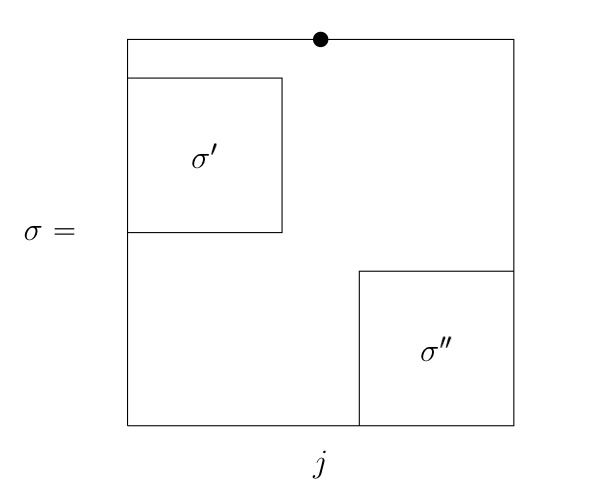
\includegraphics[scale=0.3]{./fig1/figure1.13.PNG}
    \caption{$\sigma \in \mathrm{Av}_{n}(132)$的分解}
\end{figure}
      \begin{thm}
     	$n \geqslant 0$时有
     	$$
     	\# \mathrm{Av}_{n}(132)=C(n).
     	$$
     \end{thm}
     \begin{proof}
     	利用定理1.11.2中给出的 $C(n)$的初始条件和递归关系对$n$进行归纳. 与之前一样, 我们主要关注递归公式. 取
     	$\sigma=\sigma_{1} \ldots \sigma_{n} \in \operatorname{Av}_{n}(132)$, 且设 $\sigma_{j}=n$. 故我们可记 $\sigma=\sigma^{\prime} n \sigma^{\prime \prime}$,
     	其中$\sigma^{\prime}=\sigma_{1} \ldots \sigma_{j-1}$ 且 $\sigma^{\prime \prime}=\sigma_{j+1} \ldots \sigma_{n}$.
     	显然$\sigma^{\prime}$ 与 $\sigma^{\prime \prime}$必须禁用132, 因为它们是$\sigma$的子序列. 我们还可设$\min \sigma^{\prime}>\max \sigma^{\prime \prime}$,
     	因此我们可得$\sigma$分解为图1.13所示. 事实上, 如果存在$s \in \sigma^{\prime}$ 及 $t \in \sigma^{\prime \prime}$有$s<t$, 则
     	$\sigma$包含\textsl{snt}, 而snt是132的一个副本, 矛盾. 因此$\sigma^{\prime}$ 与 $\sigma^{\prime \prime}$是排列
     	$\{n-1, n-2, \ldots, n-j+1\}$ 与 $[n-j]$, 两者都禁用132. 相反的, 如果$\sigma$的$\sigma^{\prime}, \sigma^{\prime \prime}$
     	禁用132且有图1.13中的形式, 则 $\sigma$一定禁用132. 为了完成计数, 根据我们所展示的和归纳的, $\sigma^{\prime}$有
     	$C(j-1)$ 种选择, $\sigma^{\prime \prime} $有$C(n-j)$种选择. 将它们相乘且对$j \in[n]$进行求和可得$\sigma$有$C(n)$种选择.
     \end{proof}

接下来我们将处理123, 但要证明这个我们需要一些新概念. $\sigma=\sigma_{1} \ldots \sigma_{n} \in \mathfrak{S}_{n}$的\textsl{从左到右最小值}
为满足$\sigma_{i}<\min \left\{\sigma_{1}, \sigma_{2}, \ldots, \sigma_{i-1}\right\}$的$\sigma_{i}$. 例如,
$\sigma=698371542$有从左到右最小值$\sigma_{1}=6, \sigma_{4}=3,$ 及 $\sigma_{6}=1$. 如果有必要可以区分不同的位置,
$\sigma_{j}$被称为从左到右最小值的值. 按照从左到右的顺序找出从左到右的最小值, 位置和值总是满足
\begin{equation}
    1=i_{1}<i_{2}<\cdots<i_{l} \text { and } m_{1}>m_{2}>\cdots>m_{l}=1.
\end{equation}
这里$l \geqslant 1$ .

我们需要确定, 给定一组值和位置, 是否存在具有这些从左到右最小值的排列. 为此, 我们引入了再组合学和其他领域上也很有用的组合上的
优势序位. $n$的一个\textsl{弱有序分拆}是一个非负整数序列$\alpha=\left[\alpha_{1}, \ldots, \alpha_{l}\right]$, 其中
$\sum_{i} \alpha_{i}=n$. 因此, 在弱有序分拆中0是允许的, 且我们使用0作为下标. 如果对所有$j \geqslant 1$有
$$
\alpha_{1}+\alpha_{2}+\cdots+\alpha_{j} \leqslant \beta_{1}+\beta_{2}+\cdots+\beta_{j},
$$
其中如果$j>\ell(\alpha)$时$\alpha_{j}=0$, 且$\alpha, \beta \models_{0} n$ 则 $\alpha$由$\beta$\textsl{支配},
记为$\alpha \unlhd \beta$. 对$\beta $也是相似的定义. 举个例子, [2,2,1,1]$\unlhd[3,1,2]$ 因为
 $2 \leqslant 3,2+2 \leqslant 3+1,2+2+1 \leqslant 3+1+2,$ 及 $2+2+1+1=3+1+2+0$. 由于$\alpha, \beta \models_{0} n$,
 所以最后一个不等式总是一个等式. 在下一个结果中, 读者将注意到$\iota$ 与 $\mu$的构造与(1.8)定义的映射 $\phi$.
     \begin{lem}
     	设$\sigma \in \mathfrak{S}_{n}$

       \noindent
     (1)$\sigma \in \mathrm{Av}_{n}(123)$当且仅当它的非从左到右最小值是递减的

     \noindent(2)存在$\sigma \in \mathrm{Av}_{n}(123)$的从左到右最小值的位置与值给定如(1.12)当且仅当$\iota \unlhd \mu$, 其中
      $$
      \begin{aligned}
      \iota &=\left(i_{2}-i_{1}-1, i_{3}-i_{2}-1, \ldots, i_{l+1}-i_{l}-1\right) \\
      \mu &=\left(m_{0}-m_{1}-1, m_{1}-m_{2}-1, \ldots, m_{l-1}-m_{l}-1\right)
      \end{aligned}
      $$
      且 $i_{l+1}=m_{0}=n+1$, 在这种情况下, $\sigma$是唯一的.
     \end{lem}
      \begin{proof}
     	(1)我们将证明这个命题的对偶形式.首先假设$\sigma$包含123的副本$\sigma_{i} \sigma_{j} \sigma_{k}$.
     	则$\sigma_{j}, \sigma_{k}$不可能是从左到右最小值. 因为$\sigma_{i}$在它们左边且比它们小. 又因为$\sigma_{j}<\sigma_{k}$,
     	所以非从左到右最小值序列包含一个递增. 反过来, 假设$j<k$ 时有$\sigma_{j}<\sigma_{k}$, 且它们都不是从左到右最小值.
     	令$\sigma_{i}$为 $\sigma_{j}$左边最接近的一个从左到右最小值. 这样的 $\sigma_{i}$一定存在, 因为 $\sigma$一定由一个
     	从左到右最小值开始. 因此$\sigma_{i}<\sigma_{j}<\sigma_{k}$给出123的副本.

     	(2)显然, 如果$\sigma$存在, 那么它必须是唯一的, 因为它的从左到右最小值的位置和值由(1.12)给出, 且其余元素只能按(1)的方式
     	排列. 我们可以尝试构造满足下列给定条件的$\sigma$. 在这个证明后会给出一个例子. 我们从有$n$个空位的一行开始, 现在我们在
     	位置$i_{1}<\cdots<i_{l}$填进值$m_{1}>\cdots>m_{l}$. 用降序将元素$S=[n]-\left\{m_{1}, \ldots, m_{l}\right\}$填满其余的位置
     	(非从左到右最小值的集合), 这样得到的$\sigma$禁用123, 因为 $\sigma$ 是两个递减子序列的并. 所以唯一的问题是这样做是否会导致
     	一个排列有 $m_{j}$ 作为它的从左到右最小值. 我们知道$m_{1}$总是一个从左到右最小值, 不管其他元素是什么. 现在 $m_{j+1}$是
     	$m_{j}$之后的第一个从左到右最小值当且仅当在位置$i_{j+1}$之前的空位填进了一个比$m_{j}$大的元素. 注意$\iota_{j}=i_{j+1}-i_{j}-1$
     	是位置$i_{j}$ 与 $i_{j+1}$之间的空位数量. 同样$\mu_{j}=m_{j-1}-m_{j}-1$是$m_{j}<s<m_{j-1}$的$s \in S$的数量.
     	由此可见$\iota_{1}+\cdots+\iota_{j}$是位置$i_{j+1}$之前的空位数, $\mu_{1}+\cdots+\mu_{j}$是$S$中比$m_{j}$大的数.
     	故填满空位且能保持从左到右最小值不变当且仅当满足$\iota \unlhd \mu$的不等式. 证毕.
     \end{proof}

假设我们想看是否$\sigma \in \mathrm{Av}_{9}(123)$在位置$1<4<6$有从左到右最小值$6>3>1$, 我们可以从下面看
\begin{equation}
    \sigma=6\_ \_3\_ 1\_ \_ \_.
\end{equation}
我们希望验证是否用[9]中剩余的元素以递减的顺序填满空位会得到以初始元素为从左到右最小值的排列. 一种方法是填补空位, 并验证
所需的元素是从左到右最小值:$\sigma=698371542$. 另一种方法就是使用$\iota$ 与 $\mu$ 的组合. 注意, $\iota_{1}=4-1-1=2$
是原式中$m_{1}=6$ 与 $m_{2}=3$之间的空位数, 类似$\mu_{1}=10-6-1=3$是$S=[9]-\{6,3,1\}$中比$m_{1}=6$大的元素数.
为了填补6和3之间的空位使得6是从左到右最小值, 我们使用的数字都必须大于6, 当$\iota_{1} \leqslant \mu_{1} $时这是可能的.
同样$\iota_{1}+\iota_{2} \leqslant \mu_{1}+\mu_{2}$确保可以用大于$m_{2}=3$的数字填$m_{3}=1$左边的空位, 以此类推.
故检查是否满足$\iota \unlhd \mu$也决定了 $\sigma$ 是否有正确的从左到右最小值.

我们需要一个类似引理1.12.3的$\mathrm{Av}_{n}(132)$的元素. 为了说明它, 我们定义$\alpha=\left[\alpha_{1}, \alpha_{2}, \ldots, \alpha_{l}\right]$
的弱有序分拆的\textsl{反转}为
$$
\alpha^{r}=\left[\alpha_{l}, \alpha_{l-1}, \ldots, \alpha_{1}\right]
$$
         \begin{lem}
设$\sigma \in \mathfrak{S}_{n}$
\noindent
(1)$\sigma \in \mathrm{Av}_{n}(132)$当且仅当对每一个从左到右最小值$m$, $\sigma$的右边和大于$m$的元素构成一个递增的子序列.

\noindent
(2)存在$\sigma \in \mathrm{Av}_{n}(132)$, 且有(1.12)所示的从左到右最小值的位置与值当且仅当$\mu^{r} \unlhd \iota^{r}$, 其中$\iota, \mu$由引理1.12.3给出. 这种情况下,  $\sigma$唯一.
      \end{lem}
      	 \begin{proof}
      	这一结果的证明与引理1.12.3的证明相似, 因此将留作练习. 这里我们只从它从左到右最小值与空位的式子
      	给出$\sigma \in \mathrm{Av}_{n}(132)$的构造. 同样, 在证明后会有一个例子. 我们保留之前引理证明的记号. 我们首先用元素
      	$s \in S$填满$m_{l}=1$右边的空位, 使得$m_{l}<s<m_{l-1}$按递增顺序排列且尽可能靠左(这样他们将是连续的).
      	接下来, 我们用$m_{l-1}<s<m_{l-2}$的$s \in S$来填$m_{l-1}$右边剩余的空位, 使它们形成一个递增的子序列, 且尽可能靠左.
      	继续以这种方式进行下去, 直到所有空位被填满.
      \end{proof}

假设我们希望填满(1.13), 并让 $\sigma$ 禁用132.如果$m_{3}<s<m_{2}$ 则 $s=2$, 故我们把2放在 $m_{3}=1$ 的右边可得
$\sigma=6\_ \_3\_ 12\_ \_$. 同样, 满足  $m_{1}<s<m_{2}$ 的有 $s=4,5$, 故我们将这些元素以递增顺序从左到右依次填进可得
$\sigma=6\_ \_34125\_$. 最后, 我们将比$m_{1}=6$ 大的元素用同样的方法填进可得最后的结果$\sigma=6 7 8341259$.

在我们得到$\mathfrak{S}_{3}$中所有元素都是Wilf等价的结果之前还需要最后一个概念. 假设
$\alpha=\left[\alpha_{1}, \ldots, \alpha_{l}\right]$ 和 $\beta=\left[\beta_{1}, \ldots, \beta_{l}\right]$都是$n$的弱有序分拆.
我们称$\alpha \unlhd \beta$ 当且仅当 $\beta^{r} \unlhd \alpha^{r}$. 为了证明这一点, 注意不等式
$\alpha_{1}+$ $\cdots+\alpha_{j} \leqslant \beta_{1}+\cdots+\beta_{j}$等于
$n-\left(\beta_{1}+\cdots+\beta_{j}\right) \leqslant n-\left(\alpha_{1}+\cdots+\alpha_{j}\right)$.
但$n-\left(\alpha_{1}+\cdots+\alpha_{j}\right)=\alpha_{r}+\alpha_{r-1}+\cdots+\alpha_{j+1}$, 对$\beta$也是如此.
做这个替换我们可得$\beta^{r} \unlhd \alpha^{r}$的不等式, 这里所有步骤都是可逆的. 最后我们说双射$f: S \rightarrow T$
\textsl{保持性质}$P$如果对所有$s \in S$有性质$P$等价于$f(s)$有性质$P$.
     \begin{thm}
     	$n \geqslant 0$时, 对$\pi \in \mathfrak{S}_{3}$ 有
     	$$
     	\# \operatorname{Av}_{n}(\pi)=C(n).
     	$$
     \end{thm}
     \begin{proof}
     由定理1.12.2和前面的讨论, 可以证明$\# \mathrm{Av}_{n}(123)=C(n)$. 如果我们能找到双射 $f: \mathrm{Av}_{n}(123) \rightarrow \mathrm{Av}_{n}(132)$,
     即可证明定理. 事实上, $f$会保持从左到右最小值的位置和值不变. 假设$\sigma \in \mathrm{Av}_{n}(123)$的位置和值由(1.12)给出.
     由引理1.12.3, 存在唯一$\sigma$且有$\iota \unlhd \mu$. 但正如之前提到的, 这等价于$\mu^{r} \unlhd \iota^{r}$.
     故由引理1.12.4, 存在唯一 $\sigma^{\prime} \in \mathrm{Av}_{n}(132)$的从左到右最小值有给定的位置和值, 令$f(\sigma)=\sigma^{\prime}$.
     因为$\sigma$ 与 $\sigma^{\prime}$的存在唯一性可得这是一个双射.
     \end{proof}


注意, 前面证明中对$f$的描述是很有用的. 给定$\sigma \in \mathrm{Av}_{n}(123)$, 我们去掉它的非从左到右最小值, 并使用引理
1.12.4证明中的算法重新排列它们, 因此, 用先前的例子可得$f(698371542)=678341259$.

\section{练习}
\noindent1.$n \geqslant 1$时, 用归纳法和组合学的方法来证明下列等式:
(1) $\sum_{i=1}^{n} F_{i}=F_{n+2}-1$.
(2) $\sum_{i=1}^{n} F_{2 i}=F_{2 n+1}-1$.
(3) $\sum_{i=1}^{n} F_{2 i-1}=F_{2 n}$.

\noindent2.证明如果$k, n \in \mathbb{P}$满足$k \mid n$(即$k$平均分配到$n$), 则 $F_{k} \mid F_{n}$.

\noindent3.给定$m\in \mathbb{P}$,证明斐波那契数序列是周期模$m$的;也就是说,存在$p\in \mathbb{P}$使得对所有$n\geq 0$\[
F_{n+p}\equiv F_{n}(\text{mod} m).
\]\textsl{周期模$m$}就是最小的$p$使该同余式成立。注意,对任意的$m$,寻找斐波那契序列的周期是一个公开问题。

\noindent4.\textsl{卢卡斯数}定义为$L_{0}=2$, $ L_{1}=1$, 且
$$
L_{n}=L_{n-1}+L_{n-2} \text { for } n \geqslant 2.
$$
当 $m, n \geqslant 1$时, 证明:
(1) $L_{n}=F_{n-1}+F_{n+1}$.
(2)设$\mathcal{C}_{n}$为 $n$个箱子以双方块和单方块排成一个圈的平铺, 证明$\# \mathcal{C}_{n}=L_{n}$.
(c) $L_{m+n}=F_{m-1} L_{n}+F_{m} L_{n+1}$.
(d) $F_{2 n}=F_{n} L_{n}$.

\noindent5.证明定理1.2.2.

\noindent6.验证定理1.3.1证明中两个映射是否为互逆的.

\noindent7.(1)用等式(1.5)证明定理1.3.3的(2).
(2)给出定理1.3.3中(3)的一个归纳法证明.
(3)给出定理1.3.3中(4)的一个归纳法证明.

\noindent8.设 $S$, $T$为集合.
(1)证明 $S \Delta T=(S \cup T)-(S \cap T)$
(2)证明 $(S \Delta T) \Delta T=S$
\noindent9.
\end{document}